\documentclass[11pt,a4paper]{report} 

% Für doppelseitigen Ausdruck (nur bei > 60 Seiten sinnvoll)
% \usepackage{ifthen}
% \setboolean{@twoside}{true}
% \setboolean{@openright}{true} 

% Deutsch
\usepackage[german]{babel} % deutsch und deutsche Rechtschreibung
\usepackage[utf8]{inputenc} % Unicode Text 
\usepackage[T1]{fontenc} % Umlaute und deutsches Trennen
\usepackage{textcomp} % Euro
\usepackage[hyphens]{url}
% statt immer Ab\-schluss\-ar\-beit zu schreiben
% einfach hier sammeln mit -. 
\hyphenation{Ab-schluss-ar-beit}
% Vorsicht bei Umlauten und Bindestrichen
\hyphenation{Ver-st\"ar-ker-aus-gang}
 % eigene Hyphenations, die für das Dokument gelten
\usepackage{amssymb} % Symbole
\usepackage{emptypage} % Wirklich leer bei leeren Seiten

%% Fonts, je ein kompletter Satz an Optionen

% Times New Roman, gewohnter Font, ok tt und serifenlos
%\usepackage{mathptmx} 
%\usepackage[scaled=.95]{helvet}
%\usepackage{courier}

% Palatino mit guten Fonts für tt und serifenlos
\usepackage{mathpazo} % Palatino, mal was anderes
\usepackage[scaled=.95]{helvet}
\usepackage{courier}

% New Century Schoolbook sieht auch nett aus (macht auch tt und serifenlos)
%\usepackage{newcent}

% Oder default serifenlos mit Helvetica 
% ich kann es nicht mehr sehen ...
%\renewcommand{\familydefault}{\sfdefault}

% ein bisschen eine bessere Verteilung der Buchstaben...
\usepackage{microtype}

% Bilder und Listings
\usepackage{graphicx} % wir wollen Bilder einfügen
\usepackage{subfig} % Teilbilder
\usepackage{wrapfig} % vielleicht doch besser vermeiden
\usepackage{listings} % schöne Quellcode-Listings
% ein paar Einstellungen für akzeptable Listings
\lstset{basicstyle=\ttfamily, columns=[l]flexible, mathescape=true, showstringspaces=false, numbers=left, numberstyle=\tiny}
\lstset{language=python} % und nur schöne Programmiersprachen ;-)
% und eine eigene Umgebung für Listings
\usepackage{float}
\newfloat{listing}{htbp}{scl}[chapter]
\floatname{listing}{Listing}

% Seitenlayout
\usepackage[paper=a4paper,width=14.2cm,left=36mm,height=22cm]{geometry}
\usepackage{setspace}
\linespread{1.15}
\setlength{\parskip}{0.5em}
\setlength{\parindent}{0em} % im Deutschen Einrückung nicht üblich, leider

% Seitenmarkierungen 
\newcommand{\phv}{\fontfamily{phv}\fontseries{m}\fontsize{9}{11}\selectfont}
\usepackage{fancyhdr} % Schickere Header und Footer
\pagestyle{fancy}
\renewcommand{\chaptermark}[1]{\markboth{#1}{}}
%\fancyhead[L]{\phv \leftmark}
\fancyhead[RE,LO]{\phv \nouppercase{\leftmark}}
\fancyhead[LE,RO]{\phv \thepage}
% Unten besser auf alles Verzichten
%\fancyfoot[L]{\textsf{\small \kurztitel}}
\fancyfoot[C]{\ } % keine Seitenzahl unten
%\fancyfoot[R]{\textsf{\small Technische Informatik}}

% Theorem-Umgebungen
\newtheorem{definition}{Definition}[chapter]
\newtheorem{satz}{Satz}[chapter]
\newtheorem{lemma}[satz]{Lemma} % gleicher Zähler wie Satz
\newtheorem{theorem}{Theorem}[chapter]
\newenvironment{beweis}[1][Beweis]{\begin{trivlist}
\item[\hskip \labelsep {\textit{#1 }}]}{\end{trivlist}}
\newcommand{\qed}{\hfill \ensuremath{\square}}

% Quellen teilen
\usepackage{bibtopic} 

% Hochschule Logo, noch nicht perfekt
\usepackage{hsmalogo}

% Spezialpakete
\usepackage{epigraph}
\setlength{\epigraphrule}{0pt} % kein Trennstrich

% damit wir nicht so viel tippen müssen, nur für Demo 
\usepackage{blindtext} 

% Zum Zeigen von Fehlern
\usepackage{soul}
\newcommand*\falsch{\st}

\usepackage{hyperref}
\hypersetup{
    colorlinks=true,
    linkcolor=blue,
    filecolor=magenta,      
    urlcolor=cyan,
    pdftitle={Overleaf Example},
    pdfpagemode=FullScreen,
    }

\newcommand{\tabitem}{~~\llap{\textbullet}~~}

\usepackage{xcolor}
\lstdefinestyle{customcs}{
  keywordstyle=\color{teal},
  identifierstyle=\color{violet},
  stringstyle=\color{orange}
}
 % alle Pakete und Einstellungen

%\bibliography{online}

% Hier anpassen 
\newcommand{\welchethesis}{Bachelor}
% \newcommand{\welchethesis}{Master}
\newcommand{\thesisofwas}{of Science}
\newcommand{\studiengang}{Technische Informatik}
% \newcommand{\studiengang}{Medizintechnik}
\newcommand{\titel}{Entwicklung einer Softwarelösung zur Nutzung von Smartphones als Sensor- und Aktor}
\newcommand{\kurztitel}{Template Abschlussarbeit}
\newcommand{\autor}{Marius Cerwenetz}
\newcommand{\datum}{08. Juli 2022} % Abgabedatum
\newcommand{\ort}{Mannheim}
\newcommand{\referent}{Prof.\ Dr.\ Peter Barth}
\newcommand{\korreferent}{Prof.\ Dr.\ Jens-Matthias Bohli}

\begin{document}

\begin{titlepage}
  % Kopf der Seite
  \hsmalogo[1] \hfill
  \parbox[b]{60mm}{
    % \textsf würde das Aussehen der ersten Seite ruinieren, 
    % wer will, soll das selbst außen rum machen...
    Fakultät Informationstechnik\\
    Studiengang \studiengang}
  \begin{center}
    % rumfiddeln, damit es für 4 Zeilen gerade noch so geht...
    \rule{1\textwidth}{1pt}\\[-3mm]
    \parbox[t][64mm]{110mm}{% 11 cm für Breite 13, ca. 7 für Höhe 6
      \begin{center}
        \Large{\welchethesis arbeit}\\[2mm]
        {\begin{spacing}{1.13} \huge \bfseries \titel \end{spacing}}
        \vfill
        \Large{\autor} \\[1mm] % keep space to window
        \ 
      \end{center}
    }
    \rule{\textwidth}{1pt}    
    \vfill    
    {\Large Abschlussarbeit} \\[5mm]
    {\large zur Erlangung des akademischen Grades} \\[5mm]
    {\large \welchethesis\ \thesisofwas} \\[5mm]
    \vfill    
    \begin{tabular}{ll} % Mitte der Seite
      Vorgelegt von & \autor \\
      am & \datum \\
      Referent & \referent \\
      Korreferent & \korreferent
    \end{tabular}    
    \vfill
  \end{center}
\end{titlepage}
\cleardoublepage


% Erklärung gemäß der Prüfungsordnung
\thispagestyle{empty}
\subsection*{Schriftliche Versicherung laut Studien- und Prüfungsordnung}

Hiermit erkläre ich, dass ich die vorliegende Arbeit selbstständig verfasst
und keine anderen als die angegebenen Quellen und Hilfsmittel benutzt habe.

\vspace{6em}
\noindent\begin{tabular}{p{0.37\textwidth}p{0.56\textwidth}}
\ort, \datum  & \rule{0.56\textwidth}{0.5pt}\\
              & \makebox[1cm]{\ } \autor
\end{tabular}

\vfill

\cleardoublepage

 % Titelseite, Erklärungen, etc.


\begin{abstract}
Interaktive Programmieraufgaben eignen sich besonders gut zum Programmierenlernen für angehende Programmiererinnen oder Programmierer.
Auf Mikrocontroller-Schaltungen basierende Projekte bieten durch angeschlossene Sensoren ein ideale Interaktivität, benötigen allerdings auch zusätzliches Fachwissen.
Gegenüber ihnen bietet der Einsatz von Smartphones Vorteile für Aufgaben dieser Art Vorteile gegenüber Mikrocontroller-Schaltungen.
Die Geräte bieten einen vergleichbaren Sensorumfang und können Ausgaben virtuell darstellen.
Ihre Anbindung in Programmierumgebungen ist jedoch nicht äquivalent unterstützt.
Schnittstellen zur Ansteuerung sind nicht gegeben.

Diese Arbeit behandelt die Entwicklung einer Softwarelösung namens Smartbit, welche Sensoren von Smartphones über eine Programmierumgebung ausliest und Ausgaben auf dem Smartphone ausführt.
Anforderungen an die Lösung werden anhand von Beispielaufgabenstellungen spezifiziert und für die Implementierung der Lösung berücksichtigt.
Eine Evaluation der Lösung erfolgt durch die Demonstration einer Lösung für eine Beispielaufgabe und einer Messung für drei unterschiedliche Nutzungsszenarien für angehende Programmiererinnen und Programmierer.

Die Lösung kann für den beschriebenen Einsatz verwendet werden. Die Einbindung in bestehende Programmierumgebungen ist möglich. 
Bei Aufrufen auftretende Latenzen zwischen Smartphone und Programm sind vertretbar.
\end{abstract}

\tableofcontents

\chapter{Einführung} \label{chap:intro}
Viele angehende Programmiererinnen und Programmierer mühen sich beim Programmieren lernen zum Anfang mit der Semantik von Programmiersprachen und grundlegenden algorithmischen Konzepten.
Akademische Übungsaufgaben senken durch rein virtuelle Aufgabenstellungen ohne Interaktionsmöglichkeiten die Lernmotivation.
Aufgaben in Verbindung mit Mikrocontroller-Schaltungen stellen dagegen eine praktische, fordernde und spielerische Einstiegsmöglichkeit dar, um Programmieren zu lernen.
In den Projekten werden kleine Programme realisiert, die durch die Verwendung von Sensoren Programmiererinnen und Programmierer einladen, sich an den Aufgabenstellungen auszuprobieren.
Die in Mikrocontroller-Schaltungen integrierten Sensoren sind Voraussetzung, um physikalische Eigenschaften in der realen Welt zu messen.
Von Programmiererinnen und Programmierern entwickelte Programme können auf dem Mikrocontroller die verbundenen Sensoren auslesen und auf Änderungen der gemessenen Werte reagieren.
Zusammen ermöglichen Sensoren, Mikrocontroller und das entwickelte Programm eine Bedienung der Schaltung.
Während der Entwicklung treten jedoch häufig Probleme auf.
Selten verhält sich das Programm beim ersten Versuch korrekt.
Eine Anpassung des Codes ist nötig, bis das Fehlverhalten beseitigt ist.
Diese kontinuierliche Weiterentwicklung mindert Ängste vor Code-Änderungen, schafft Routine in der Entwicklung und damit ein tieferes Verständnis und Hintergrundwissen für die Problemstellung.
Sinnvoll sind diese Projekt-Eigenschaften insbesondere für Programmiererinnen und Programmierer mit wenig Vorwissen, wie Schüler oder Erstsemester-Studierende.
Praktische Programmieraufgaben bieten für sie den größten Lerneffekt und motivieren am Meisten \cite{learning_computer_programming}.

Mikrocontroller-Projekte benötigen allerdings teure Einstiegs-Kits.
Die Kosten eines Arduino-Development-Boards belaufen sich im Arduino-Shop über 80,00 € \cite{arduino_kit}.
Ein Großteil der Kosten entfällt zwar auf den konkreten Mikrocontroller, ein nicht unerheblicher Teil jedoch auf Peripherie wie wie Breadboards, Verbindungskabel und Erweiterungsboards.
Die Peripherie-Anbindung setzt zusätzliches Hintergrundwissen in elektrotechnischen Bereichen voraus, zum  Beispiel bei den Verschaltungskonventionen von Breadboards oder der Benutzung von Lötkolben.
Fehlerhafte Verdrahtungen oder ein Fehlgebrauch resultieren in zerstörten Komponenten oder Verletzungen.
Dies stellt ebenfalls eine Einstiegshürde dar, die die eigentliche interaktive Lernerfahrung herauszögert und die Motivation senkt.

Smartphones dienen für angehende Programmiererinnen und Programmierer als Alternative zu herkömmlichen Mikrocontroller-Schaltungen für Programmieraufgaben.
Ein Vorteil ihrer Nutzung gegenüber Mikrocontrollern bei Programmierprojekten liegt in der Verfügbarkeit.
2022 besaßen weltweit 5,2 Mrd. Menschen ein Smartphone \cite{smartphone_users}.
Sie sind insbesondere unter Jugendlichen und jungen Erwachsenen weit verbreitet.
Im Alltag wird es für Chats, Social-Media oder Spiele verwendet.
Sie sind also häufig bereits in Gebrauch und müssten für die Nutzung von Programmierprojekten nicht zusätzlich beschafft werden.
Projekte in denen Smartphones statt Mikrocontroller verwendet werden reduzieren das Risiko eines Verdrahtungsfehlers der Schaltung dadurch, dass elektrische Schaltungen bereits intern gefertigt und somit von äußerlicher Fehlverwendung geschützt sind.
Der Sensoren-Umfang ist vergleichbar mit dem von Mikrocontrollern.
In Smartphones sind zahlreiche Sensoren wie Lagesensoren, Gyroskop oder Annäherungssensoren integriert.
Durch diese können sie zuverlässig physikalische Umgebungseigenschaften messen.
Neben kabelgebundenen Übertragungsschnittstellen wie USB oder Lightning besteht auch die Möglichkeit, drahtlose Verbindungsmöglichkeiten wie WLAN oder Bluetooth zu nutzen.
Die Geräte sind zudem batteriebetrieben, was Lösungen ermöglicht, die von einer Spannungsversorgung unabhängig sein können. 
Eine Einbindung von Smartphones in Entwicklungsumgebungen ist in den meisten Fällen jedoch nicht möglich.
Visuelle und haptische Ausgaben auf dem Smartphone erfordern eine mobile Anwendung, da Smartphone-Betriebssysteme keine nativen Ausgabemethoden bieten.

In dieser Arbeit wurde eine Softwarelösung mit dem Namen Smartbit entwickelt.
Sie ermöglicht Smartphones statt Mikrocontroller-Schaltungen für die Entwicklung von interaktiven Projekten zu nutzen. 
Sensoren sollen ausgelesen und Ausgaben auf dem Smartphone ausgelöst werden können.
Für die Verwendung der Smartbit-Lösung werden angehenden Programmiererinnen und Programmierern Beispielaufgaben dargereicht, deren Bewältigung eine Bereitstellung von Benutzungsmöglichkeiten seitens der Smartbit-Lösung erfordert.
Die Aufgaben, sowie aus ihnen ableitbare Anforderungen und Rahmenbedingungen, sind in Kapitel \ref{chap:Experimente} zu aufgeführt.
Die drei Komponenten Smartphone-App, Kontrollanwendung und Programmierumgebung und werden in Kapitel \ref{chap:architektur} vorgestellt.
Damit die Komponenten zusammenarbeiten können müssen sie Nachrichten austauschen.
Die Einsatzzwecke der Nachrichtentypen und der Nachrichtenaustausch werden in Kapitel \ref{chap:message_formats} erklärt beziehungsweise exemplarisch veranschaulicht.
Einbindung und Nutzung der Schnittstellen der Programmierumgebung werden in Kapitel \ref{chap:libs} erklärt.
Der Aufbau und das Verhalten, der zwischen Smartphone-App und Programmierumgebung vermittelnden Kontrollanwendung, wird in Kapitel \ref{chap:server_software} erklärt.
Kapitel \ref{chap:app} behandelt die Funktionsweise und den Aufbau der Smartphone-App im Detail.
In Kapitel \ref{chap:eval} wird untersucht, ob die vorgegebenen Anforderungen erfüllt wurden.
Dort wird zudem die Verwendung der Smartbit-Lösung anhand einer Beispielaufgabe vorgestellt.
Bei der Entwicklung aufgetretene Schwierigkeiten, Verbesserungsvorschläge und Erweiterungsmöglichkeiten der Smartbit-Lösung werden in Kapitel \ref{chap:fazit} diskutiert.

\chapter{Smartphones als Mikrocontroller-Ersatz für Programmieraufgaben} \label{chap:Experimente}
Smartphones sind in sich geschlossene, technische Geräte, die neben vordefinierten Verbindungsschnittstellen wie einem USB- bzw. Lightning-Port, WLAN und Bluetooth keine weiteren Schnittstellen bieten, um externe Hardware und Schaltungen anzuschließen.
Gegenüber Mikrocontroller-Schaltungen bieten sie jedoch einen vergleichbaren Sensorumfang.
Integrierte Lautsprecher können die in einer Mikrocontroller-Schaltung  manuell angeschlossenen Piepser ersetzen.
Zudem müssen Smartphones bei Ausgaben nicht auf Mehrzweck-Ausgabemöglichkeiten wie LED-Grids zurückgreifen, da zweckgebundene UI-Elemente wie Textfelder, Textausgaben oder Bildausgaben während der App-Entwicklung beliebig platziert werden können.

In diesem Kapitel werden Beispielprogrammieraufgaben vorgestellt.
Diese können sowohl mit Mikrocontroller-Schaltungen, als auch mit der in dieser Arbeit implementierten Smartbit-Lösung gelöst werden.
Des Weiteren werden die aus den Beispielprogrammieraufgaben hervorgehenden Anforderungen aufgestellt und erörtert.

\section{Beispielprogrammieraufgaben}\label{sec:activities}
Praxisnahe Programmieraufgaben motivieren mit interessanten Aufgabenstellungen Programmiererinnen und Programmierer.
Die in diesem Abschnitt vorgestellten Beispielaufgaben definieren das von Sensormesswerten abhängige Verhalten interaktiver Programme.
Die Aufgabenstellungen sind in Tabelle \ref{tab:excercises} aufgeführt.
Für jede Aufgabe werden die benötigen Sensortypen und Ausgabeschnittstellen beschrieben.
Leserinnen und Leser werden in der Entscheidungsfindung durch die Angabe eines dreistufigen Schwierigkeitsgrades unterstützt.
Dies soll verhindern, dass sich unerfahrene Programmierer zu Anfang mit komplizierten Aufgaben überfordern.
\begin{table}[htbp]
  \centering
  \begin{tabular}{|l|c|p{2.3cm}|c|}
      \hline
      \textbf{Name der Aufgabe} & \textbf{Benötigte Sensoren} & \textbf{Verwendete Ausgabeschnittstellen} & \textbf{Schwierigkeitsgrad} \\
      \hline
      Disco & - & LED & Einfach \\
      \hline
      Würfeln & Lagesensor & Textfeld & Einfach \\
      \hline
      Diebstahl-Alarm & Annäherungssensor & Textfeld, LED, Vibration & Mittel \\
      \hline
      Klatsch-Zähler & Mikrofon & Textfeld & Mittel \\
      \hline
      Dreh-Zähler & Lagesensor & Textfeld & Schwer \\
      \hline
  \end{tabular}
  \caption{Beispielprogrammieraufgaben}
  \label{tab:excercises}
\end{table}

In der Aufgabe \textit{Disco} soll eine virtuelle LED für eine Zeitdauer von 500 ms grün und anschließend 500 ms rot leuchten.
Sensoren werden in dieser Aufgabe nicht verwendet, da die LED-Ausgabe unabhängig von Sensormesswertänderungen ausgeführt wird, weshalb Aufgabe als \textit{Einfach} eingestuft wird.

In der Aufgabe \textit{Würfeln} soll ein Schütteln des Geräts erkannt werden.
Verwendet wird ein Gerätebeschleunigungen messender Lagesensor.
Wird ein Schütteln erkannt, soll auf dem PC eine Zufallszahl generiert werden.
Anschließend wird diese auf dem Endgerät in einem Textfeld ausgegeben.
Der Schwierigkeitsgrad wird ebenfalls auf \textit{Einfach} eingeschätzt, da die Aufgabe unter Verwendung lediglich eines Sensors und einer Ausgabe lösbar ist.

In der Aufgabe \textit{Diebstahl-Alarm} wird unter Verwendung des Näherungssensors das örtliche Umfeld des Geräts auf eine Annäherung überprüft.
Im Falle einer Annäherung wird ein alarmierender Text im Textfeld ausgegeben.
Zusätzlich soll die LED die wie in Aufgabe \textit{Disco} die Farbe wechseln.
Neben den visuellen Ausgaben wird die Vibrationsfunktion als haptisches Feedback benötigt, die das Gerät fünf mal für 1000 ms vibrieren lässt.
Der Schwierigkeitsgrad der Aufgabe ist als \textit{Mittel} eingestuft, da hier zwischen Alarm- und Normalzustand unterschieden werden muss.
Entfernt sich eine Person, muss der Alarm-Zustand verlassen und alle Ausgaben auf ihren Initialwert zurückgesetzt werden.

Bei der Aufgaben \textit{Klatsch-Zähler} muss für einen selbstdefinierten Zeitraum die Anzahl der Händeklatscher gemessen werden.
Diese Anzahl wird anschließend im Textfeld des Geräts ausgegeben.
Verwendet werden das Mikrofon als Ein- und das Textfeld als Ausgabe.
Die Schwierigkeit ist auf \textit{Mittel} angesetzt, da die Messwerte von Händeklatschern unterschiedliche Intensitäten aufweisen.
Um einen Händeklatscher zu identifizieren, ist es nötig Grenzwerte zu ermitteln um sie von normalen Hintergrundgeräuschen abzugrenzen.
Eine Visualisierung der Messdaten kann bei dieser Aufgabe helfen.

In  der Aufgabe \textit{Drehzähler} soll der Programmierer das Device innerhalb eines selbstdefinierten Zeitraums drehen und ein Programm entwickeln, das anhand der Messdaten die Anzahl der Umdrehungen ermittelt.
Diese Anzahl soll anschließend im Textfeld auf dem Gerät ausgegeben werden.
Verwendet werden hier ebenfalls der Lagesensor als Sensoreingabe und das Textfeld als Ausgabe.
Die Aufgabe ist als \textit{Schwer} bewertet, da hier Wiederholungen in einer Werteabfolge erkannt werden müssen, welche jedoch wie bei der Aufgabe \textit{Klatsch-Zähler} in ihrer Größe variieren können.
Abhängigkeiten zwischen den Messwertergebnissen erschweren eine Erkennung der Umdrehungen zusätzlich.

\section{Anforderungen an Smartbit}\label{sec:anforderungen}
Aus der vorangegangenen Beschreibung von Beispielaufgaben lassen sich Anforderungen an die Smartbit-Lösung ableiten.
Die Zielgruppe besteht, wie in der Einleitung beschrieben, aus informatik-affinen Studieninteressierten oder angehenden Programmiererinnen oder Programmierern, mit Hauptfokus auf sich im Grundstudium befindende Studierende der Fakultät Informationstechnik der Hochschule Mannheim.
Voraussetzung der Nutzung der App ist der Besitz eines PCs und eines Android-Smartphones  mit Internetzugang.

Anhand der Beispielaufgaben werden Anwendungsfälle spezifiziert, die die Nutzeranforderungen definieren.
Eine Übersicht der Anwendungsfälle ist in Abbildung \ref{fig:usecase} dargestellt.
\begin{figure}[htbp]
  \centering
  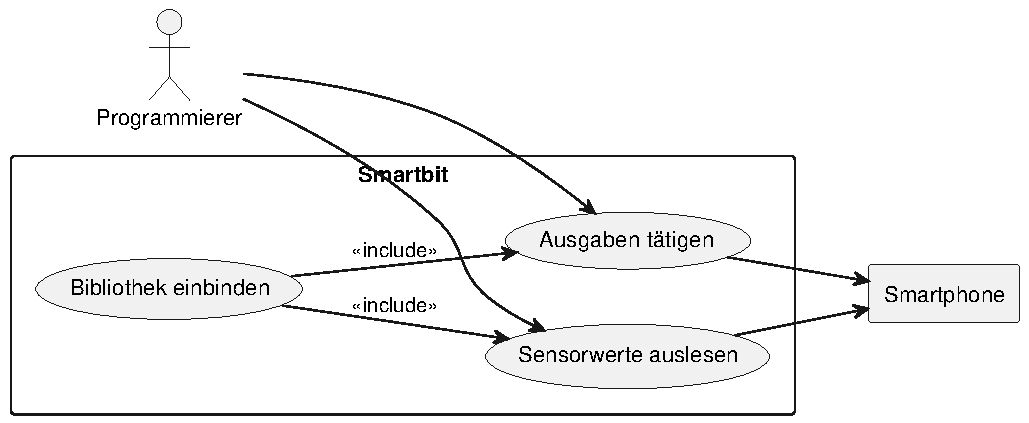
\includegraphics[width=.8\textwidth]{images/usecase_usage.pdf}
  \caption{Anwendungsfälle für die Benutzung der Lösung}
  \label{fig:usecase}
\end{figure}
Nutzerinnen und Nutzer möchten durch die Smartbit-Lösung Ausgaben auf dem Smartphone tätigen und Sensorwerte des Smartphones auslesen können.
Ausgaben sollen visuell über ein Textfeld und eine LED, und haptisch über eine Vibrationsausgabe möglich sein.
Sensor-Anfragen sollen, zur Erfüllung der Aufgaben, für den Lage- und Annäherungssensor sowie dem Mikrofon möglich sein.
Für die Bedienung aller Ausgabemöglichkeiten und der Abfrage der spezifizierten Sensortypen, muss eine in bestehenden Programmcode einbindbare Funktion existieren.
Die Verwendung der Lösung soll verständlich und ohne viel Vorwissen möglich sein.
Auf serialisierte Ausgabeformate ist zu verzichten.
Funktionen müssen Rückgabewerte in Form von primitiven Datentypen zurückgeben.
Um die Kompatibilität mit, von Programmiererinnen oder Programmierern entwickelten Programmen, zu erhöhen, müssen die Funktionen in mehreren Programmiersprachen zur Verfügung stehen.
Smartbit soll für Nutzerinnen und Nutzer, neben der Einbindung in Programme, auch leicht in Entwicklungsumgebungen integrierbar und mit wenig Boilerplate-Code verwendbar sein.
Der Einsatz der Entwicklungsumgebung Eclipse IDE \cite{eclipse-ide} ist an der Fakultät Informationstechnik der Hochschule Mannheim weit verbreitet und wird in den Lehrveranstaltungen des Grundstudiums umfassend genutzt.
Es ist davon auszugehen, dass Studierende mit der Benutzung dieser Entwicklungsumgebung vertraut sind.
Die Smartbit-Einbindung soll daher insbesondere für Eclipse IDE unterstützt werden.
Da es sich um eine plattformunabhängige \acrfull{ide} handelt, muss auch die Smartbit-Lösung plattformübergreifend, also für Unix und Windows-Systeme, in diese Entwicklungsumgebung eingebunden werden können.

Um die Benutzbarkeit und Effizienz sicherzustellen, muss die Smartbit-Lösung ein responsives Verhalten aufweisen.
Responsivität trägt zur Lernerfahrung bei, da sich physikalische Änderungen unmittelbar auf das Verhalten des entwickelten Programms auswirken.
Latenzen werden durch die \acrfull{rtt} gemessen.
Diese beschreibt die Zeitdauer der Übermittlung einer Nachricht über Hin- und Rückweg eines Hosts zu einem Anderen.
Initial müssen Sensordaten vorliegen, um Sie vom Smartphone zu übermitteln.
Das Starten von Sensormessprozessen erfordert jedoch Zeit, was die Latenzen erhöht. 
Smartphones bieten keine kabelgebunden Netzwerkschnittstellen, so dass drahtlose Netzwerke genutzt werden müssen.
Der Versand der Sensorwerte wird durch den Transportweg zwischen Smartphone und Programmierumgebung und deren lokale Gegebenheiten verzögert.
Latenzzeiten können je nach Mobilfunk- bzw WLAN-Standard, Umwelteinflüssen und der Anzahl der registrierten Geräte in Funkzellen variieren.
Kollisions-Präventionsprinzipien wie \acrfull{csmaca} verhindern bei WLAN-Verbindungen zwar, das Geräte gleichzeitig senden, erhöhen dadurch allerdings die Latenzen.
% Gelöst durch Puffer
Die Latenzen sind ebenfalls abhängig vom Standard des mobilen Netzwerks.
Bei WLAN 802.11b beträgt die Latenz ca. 10 ms, kann jedoch beispielsweise bei Verbindungen mit \acrfull{umts} auf 300 ms bis 400 ms ansteigen \cite{network_latencies}.
Zudem fällt die Reaktionszeit bei mehreren Sendungen unterschiedlich aus, was bei einer synchronen Übertragung zu für Nutzer nicht nachvollziehbaren Verzögerungen führt.
% Gelöst durch Puffer
Bei der Übertragung von Sensormessdaten ist auf den Gebrauch ihrem Einsatzzweck entsprechender Protokolle zu achten.
Um die Sicherheit zu erhöhen müssen Nachrichten auf den Transportwegen verschlüsselt übertragen und eine Ausführung von Schadcode auf dem Smartphone verhindert werden.
Bei der Kommunikation zwischen Smartphone-Anwendung und Programmierumgebung kann es zu Komplikationen kommen.
Um die Wartbarkeit zu gewährleisten, müssen Smartbit-Abläufe transparent sein.
Die Lösung muss Nachrichtenabläufe nachvollziehbar darstellen, um fehlerhafte Konfigurationen zu vermeiden.

\chapter{Smartbit-Architektur und Spezifikation} \label{chap:architektur}
In diesem Kapitel werden die Komponenten der Smartbit-Lösung vorgestellt und ihr Verhalten spezifiziert.
Der Fokus liegt auf den zur interkomponellen Kommunikation verwendeten Protokollen und den Anforderungen berücksichtigenden Designentscheidungen zur Implementierung der Lösung.
Spezifiziert wird das Verhalten der Lösung exemplarisch anhand des Ablaufs eines Funktionsaufrufs.

Smartbit besteht aus den drei Komponenten Programmierumgebung, Kontrollprogramm und Android-Anwendung, die zur korrekten Funktionsweise miteinander kommunizieren.
Eine Übersicht des Aufbaus ist in Abbildung \ref{fig:design} dargestellt.
\begin{figure}[htbp]
\centering
% 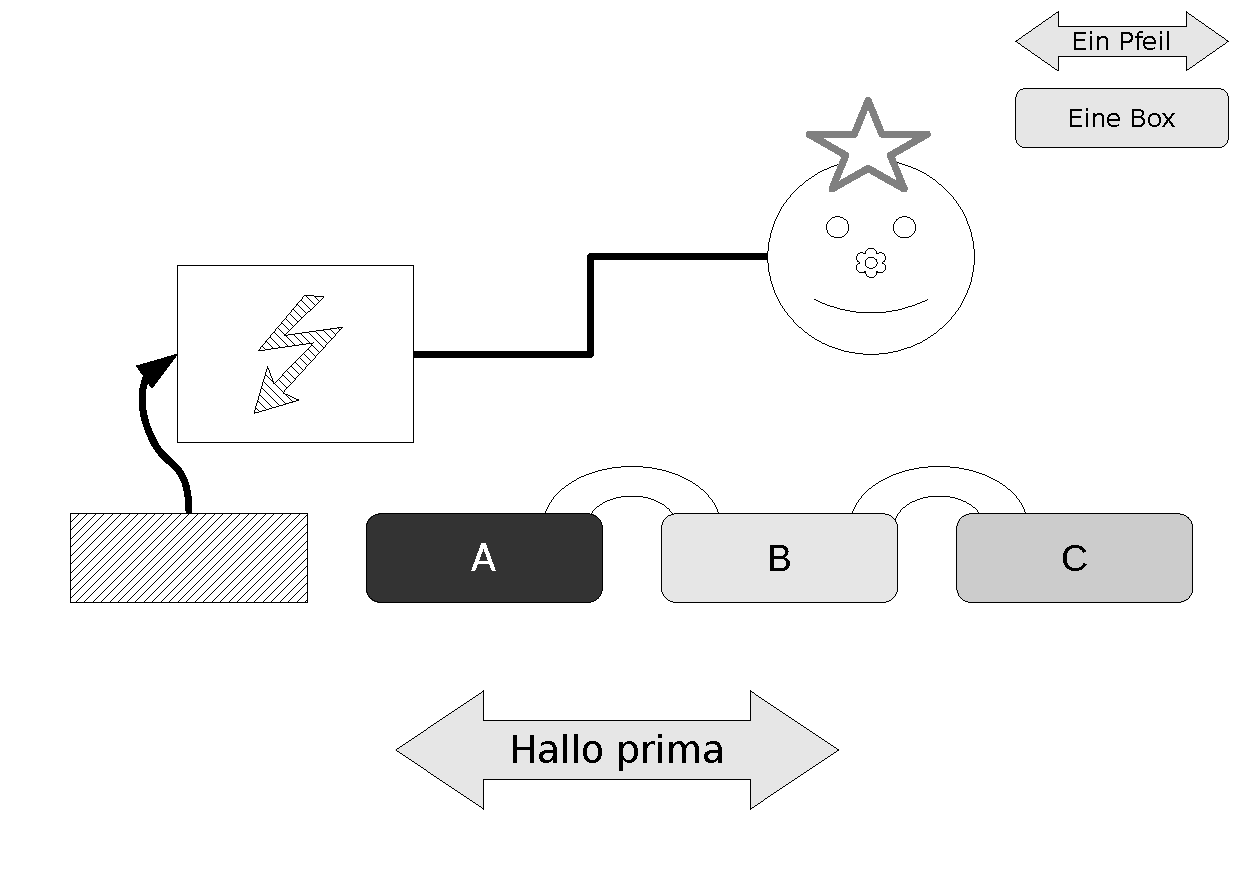
\includegraphics[width=.8\textwidth]{zeichnung.eps}
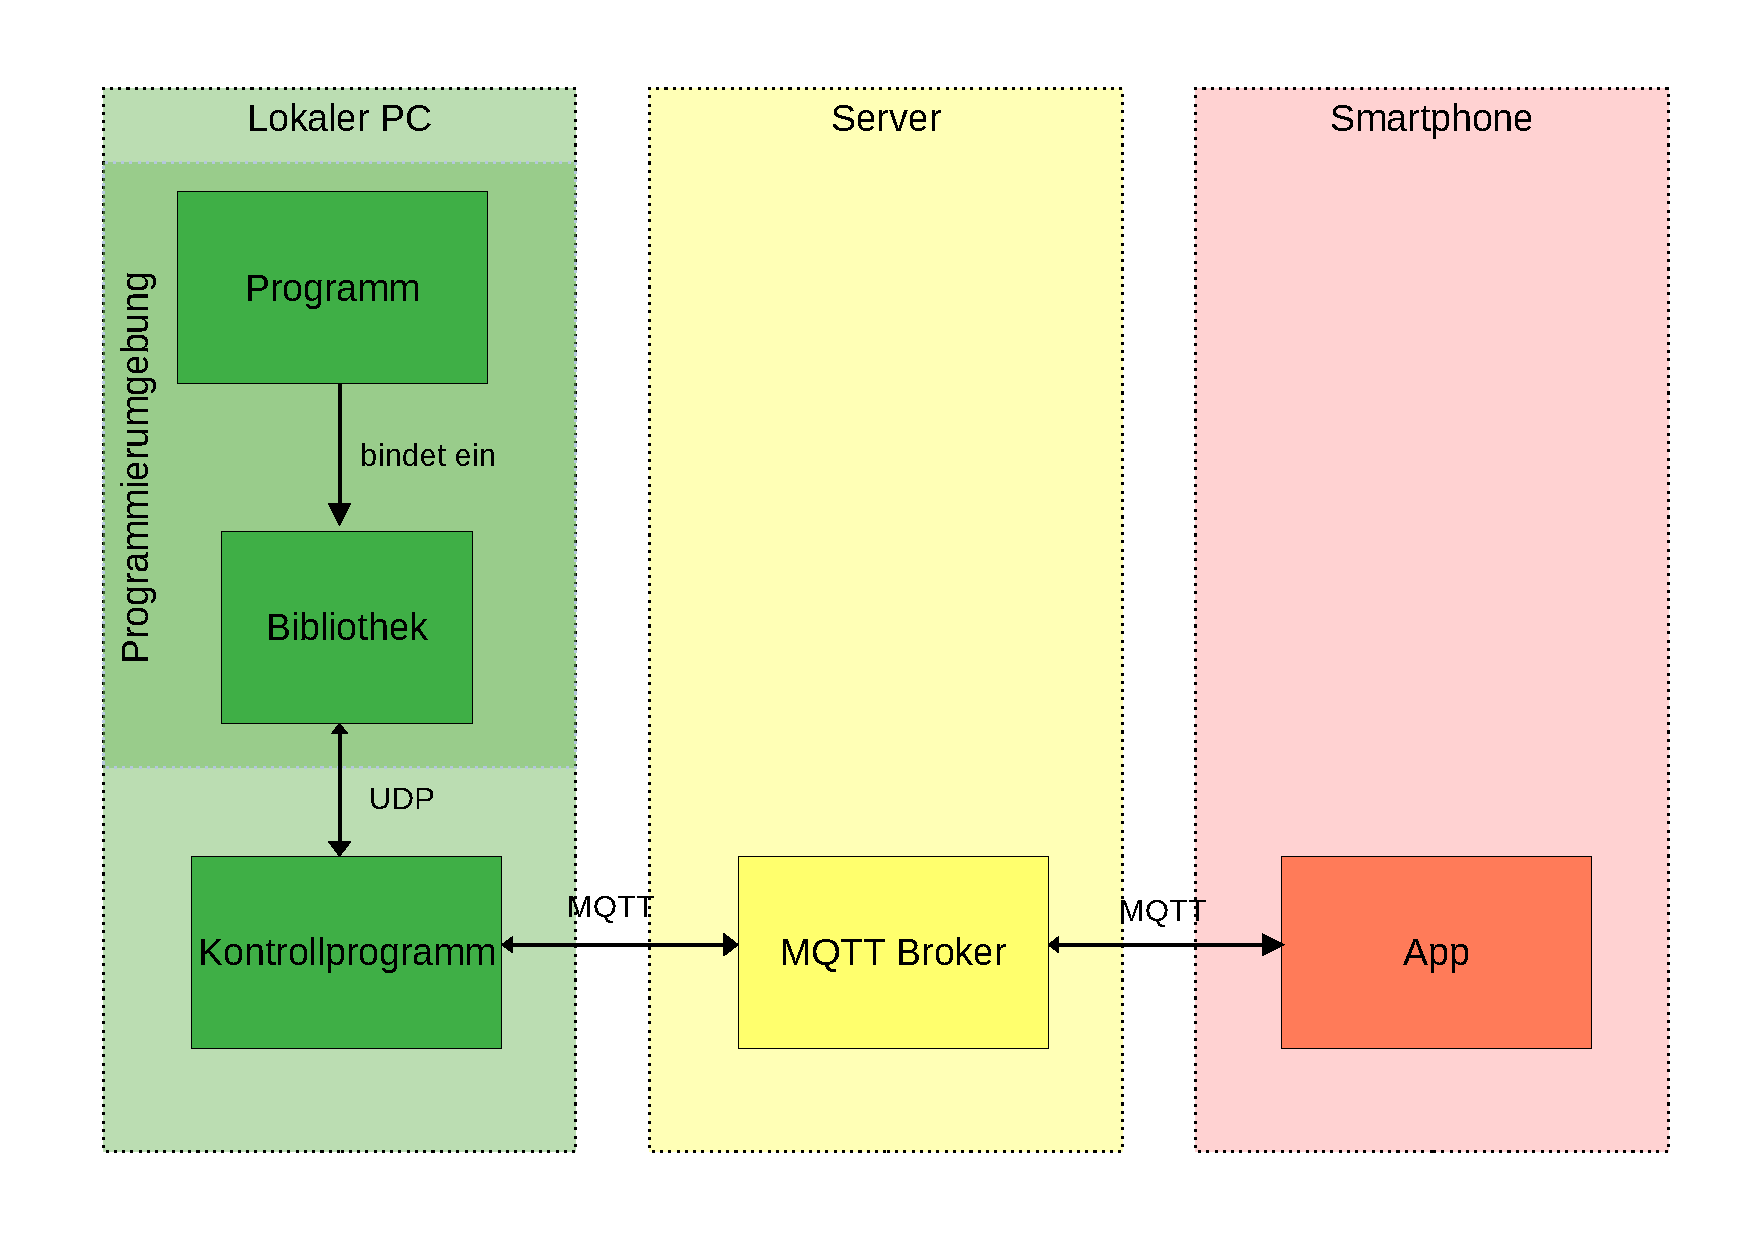
\includegraphics[width=\textwidth]{images/framework.pdf}
\caption{System-Aufbau}
\label{fig:design}
\end{figure}
Um mit dem Smartphone zu interagieren bietet die Programmierumgebung eine programmiersprachenunabhängige Bibliothek mit Schnittstellen in Form von Stub-Funktionen an, die die \acrfull{api} der Kontrollanwendung nutzen.
Die Bibliothek kann in bestehenden Programmcode eingebunden werden um die angebotenen Funktionen zu verwenden.
Die in der Programmiersprache Python implementierte Kontrollanwendung, welche ebenfalls auf dem lokalen PC betrieben wird, dient der Nachrichtenvermittlung zwischen Smartphone-App und Programmierumgebung.
Latenzen zwischen Smartphone und Programmierumgebung werden durch den Einsatz eines Zwischenpuffers für Sensorwerte vor der Programmiererin oder dem Programmierer verschleiert.
Schwankende Übertragungsgeschwindigkeiten, die durch kabellose Netzwerkschnittstellen verursacht werden, werden somit umgangen.
Das Zwischenspeicher ist ebenfalls Aufgabe der Kontrollanwendung.
Ausgabemöglichkeiten werden von der für Android-Smartphones implementieren mobilen Anwendung angeboten.
Die Anwendung reagiert auf von Funktionen der Bibliothek aufgerufenen Ausgabe-Anfragen und sendet kontinuierlich Sensorwerte zur Zwischenspeicherung an die Kontrollanwendung.
Zur Reduktion der Latenzzeiten beim Start der Sensormessprozesse werden diese bereits zum Start der Anwendung ausgeführt, so dass die Kontrollanwendung bereits vor der Ausführung des Programms der Programmiererin oder des Programmierers auf Sensorwerte zurückgreifen kann.
Die Komponenten stehen untereinander in einer 1:1-Beziehung.
Programmiererinnen und Programmierer können mit \textit{einem} Programm und \textit{einer} Kontrollanwendung \textit{ein} Smartphone ansteuern.
Für das Ansteuern mehrerer Smartphones wird jeweils eine Kontrollanwendung benötigt.

Zur Übermittlung der Nachrichten werden die Protokolle \acrfull{mqtt} und \acrfull{udp} eingesetzt.
MQTT ist ein auf einem Observer-Pattern basierendes Client-Server-Protokoll.
Durch einen 2 Byte großen Header und eine maximale Payload-Größe von 260 MB \cite{mqtt-size} ist es leichtgewichtig und gleichzeitig flexibel.
Nachrichten werden zur Publizierung auf einem Topic an einen MQTT Broker gesendet.
Dieser leitet sie dann an alle Clients weiter die das Topic abonniert haben.
Die Verwendung von MQTT ist vom Referenten vorausgesetzt.
Die UDP-Kommunikation zwischen Bibliothek und Kontrollprogramm auf dem lokalen PC wird über ein Loopback-Interface umgesetzt um die Latenzzeiten zwischen Programmierumgebung und Kontrollprogramm zu minimieren.
Das Loopback-Interface ist eine virtuelle Netzwerk-Schnittstelle des Betriebssystems eines PCs.
Pakete werden nicht über externe Netzwerk-Schnittstellen wie Netzwerkkarten versendet, sondern verbleiben im Netzwerk-Stack des Betriebssystems.
Zwischen Programmierumgebung und Kontrollanwendung auftretende Latenzen betragen weniger als eine Millisekunde.
Zur weiteren Minimierung der Latenzen wird UDP als verbindungsloses Protokoll eingesetzt.
Die Verwendung verbindungsorientierter Protokolle wie TCP würde neben ihrer Übertragungssicherheit durch eine größere Anzahl an zu sendenden Nachrichten die Latenzen erhöhen.
Da ein Übertragungsfehler lediglich den Verlust einer Sensormesswert-Anfrage bedeutete ist eine Reduktion der Übertragungssicherheit zwischen Bibliothek und Kontrollanwendung annehmbar.  
Als Nachrichtenformat wird \acrfull{json}verwendet.
Das menschenlesbare, kompakte Nachrichtenformat ist weit verbreitet und wird von vielen Softwarebibliotheken unterstützt.
Es unterstützt die Darstellung von Zahlen, Strings, Booleans und Arrays als Schlüssel-Wert-Paare und ermöglicht eine Schachtelung von Objekten.
Als Character-Encoding kommt UTF-8 zum Tragen, was beispielsweise eine Übertragung von Emojis ermöglicht.

Die beschrieben Komponenten bieten ein heterogenes verteiltes System, das über Nachrichten kommuniziert.
Um das von den Nachrichten abhängige Verhalten der Komponenten zu spezifizieren, wird im Folgenden der Ablauf einer Beispielnachricht vorgestellt.
In Abbildung \ref{fig:arch_flow} ist eine schematische Darstellung der Funktionsweise einer Ausgabe-Funktion abgebildet.
Dies könnte beispielsweise eine Funktion sein, die einen Text auf dem Textfeld anzeigen soll.
\begin{figure}[htbp]
  \centering
  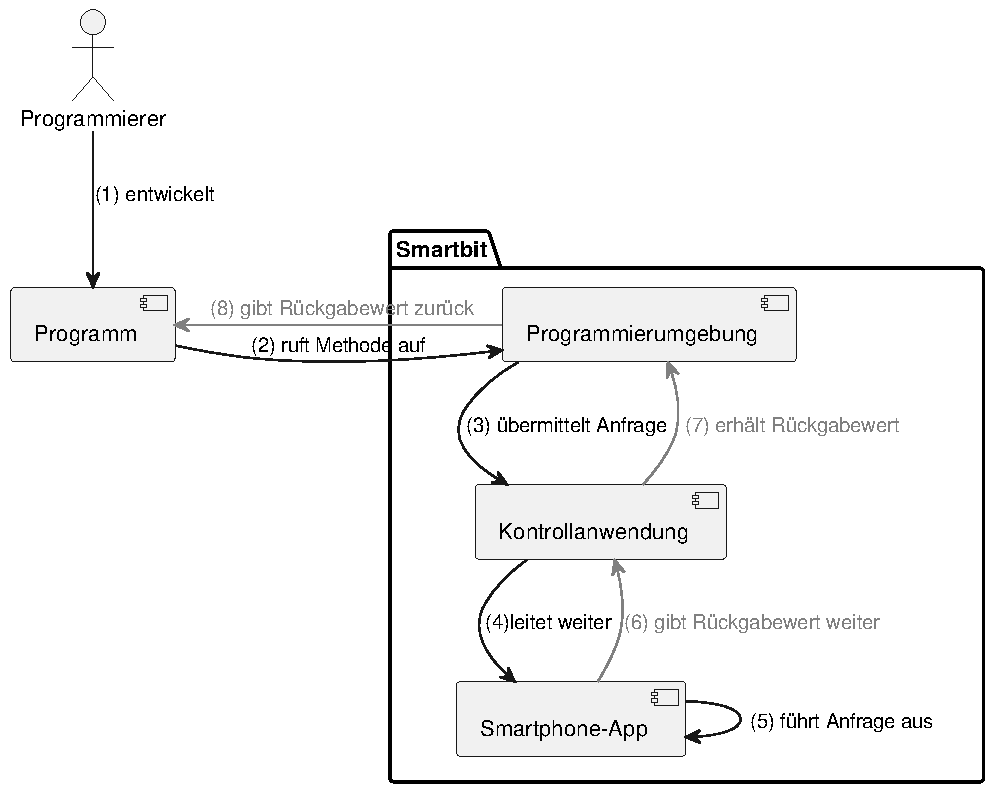
\includegraphics[width=\textwidth]{images/arch_call_flow.pdf}
  \caption{Nachrichtenablauf}
  \label{fig:arch_flow}
\end{figure}
Die Bibliothek mit den, zur Interaktion mit dem Smartphone geeigneten, Stub-Funktionen kann in Programmcode der Programmiersprachen C, Java und Python eingebunden werden (1).
Führt eine Programmiererin oder ein Programmierer einen Funktionsaufruf der Bibliothek aus (2), übermittelt die Bibliothek eine Anfrage per MQTT an das Kontrollprogramm (3).
Dieses entscheidet über die weitere Verfahrensweise.
Anfragen, die Sensormessdaten des Smartphones fordern, werden direkt bedient.
Dieser Weg ist in der Abbildung nicht dargestellt.
Ausgabe-Anfragen werden per MQTT an das Smartphone übertragen (4).
Die Smartphone-App nimmt die Anfrage an und führt Sie aus (5).
Es gibt Ausgaben die Rückgabewerte zurückgeben.
Ihr Ablauf ist in der Abbildung grau dargestellt.
In diesem Fall sendet die App den Rückgabewert an die Kontrollanwendung (6), welche ihn an die Bibliothek weiterleitet (7).
Die Bibliothek gibt den Rückgabewert zum Schluss an die Bibliothek zurück (8)


\chapter{Nachrichtenformate der Komponenten}\label{chap:message_formats}
Ein einheitliches Nachrichtenformat ist Voraussetzung für den Nachrichtenaustausch.
Der ausgearbeitete Nachrichtenstandard definiert die Nachrichten in einem Klartextformat.
Nachrichten-Vorlagen sind in einer Datei gespeichert und werden in der Bibliothek, dem Kontrollprogramm und in der Smartphone-App eingelesen, wodurch Sie in allen Komponenten kongruent vorliegen.
Es gibt unterschiedliche Nachrichtentypen, welche in Tabelle \ref{tab:message_types} aufgeführt sind.
Zur besseren Nachvollziehbarkeit der Kommunikation sind zusätzlich Quelle, Ziel und das verwendete Netzwerkprotokoll angegeben.
Eine Liste der vollständigen Nachrichtentypen, inklusive ihrer Felder, ist im Anhang aufgeführt.
\begin{table}[htbp]
  \centering
  \begin{tabular}{|l|p{30mm}|c|c|}
      \hline
      \textbf{Nachrichtentyp} & \textbf{Quelle} & \textbf{Ziel} & \textbf{Netzwerkprotokoll}\\
      \hline
		sensor\_request & Bibliothek & Kontrollprogramm & UDP\\
       \hline
       sensor\_response & Kontrollprogramm & Bibliothek & UDP\\
       \hline
		update\_request & Smartphone & Kontrollprogramm & MQTT\\
       \hline
		rpc\_request & Bibliothek, Kontrollprogramm & Smartphone & UDP/MQTT\\
       \hline
		rpc\_response & Smartphone, Kontrollprogramm & Bibliothek & UDP/MQTT\\ 
       \hline
  \end{tabular}
  \caption{Nachrichten-Typen}
  \label{tab:message_types}
\end{table}

\texttt{Sensor\_requests} kommen bei Sensormesswert-Abfragen zum Einsatz.
Dieser Nachrichtentyp wird von der Bibliothek an das Kontrollprogramm gesendet, wo die vom Smartphone übermittelten Sensorwerte zwischengespeichert wurden.
Nach Eingang ermittelt das Kontrollprogramm, durch Angabe des gewünschten Sensortyp-Kürzels im Feld \texttt{sensor\_type}, den gespeicherten Sensormesswert.
Sensortyp-Kürzel sind für alle Sensoren definiert und dienen in der Kontrollanwendung als Schlüssel der Adressierung der Messwerte im Key-Value-Speicher.
Die Kürzel sind in Tabelle \ref{tab:sensor_types} aufgelistet. 
\begin{table}[htbp]
  \centering
  \begin{tabular}{|c|c|}
      \hline
      \textbf{TYPE-Kürzel} & \textbf{Beschreibung} \\
      \hline
      accel\_\{x,y,z\} & Lagesensor für die X, Y oder Z-Richtung \\
      \hline
       gyro\_\{x,y,z\} & Gyroskop-Sensor für die X, Y oder Z-Richtung \\
      \hline
      prox & Näherungssensor \\
      \hline
  \end{tabular}
  \caption{Sensor-Kürzel mit Beschreibung}
  \label{tab:sensor_types}
\end{table}
Ist für den Sensortyp ein Sensormesswert im Key-Value-Store vorhanden, wird das Ergebnis in einer \texttt{sensor\_response}, im Feld \texttt{sensor\_value}, zurückgesendet.
Die Antwort wird von der Bibliothek angenommen und an die aufrufende Funktion zurückgegeben.
Um stets aktuelle Sensormesswerte zu erhalten, müssen sie vom Smartphone in regelmäßigen Zeitabständen übermittelt werden.
Die Android-App sendet daher in periodischen Abständen Nachrichten des Typs \texttt{update\_request} an das Kontrollprogramm.
Übermittelt werden zur Einspeicherung und Zuordnung im Key-Value-Store sowohl der Sensortyp als auch der Sensormesswert.
Der gesamte Ablauf der Sensordatenübertragung ist in Abbildung \ref{fig:message_flow_requests} dargestellt.
\begin{figure}[htbp]
\centering
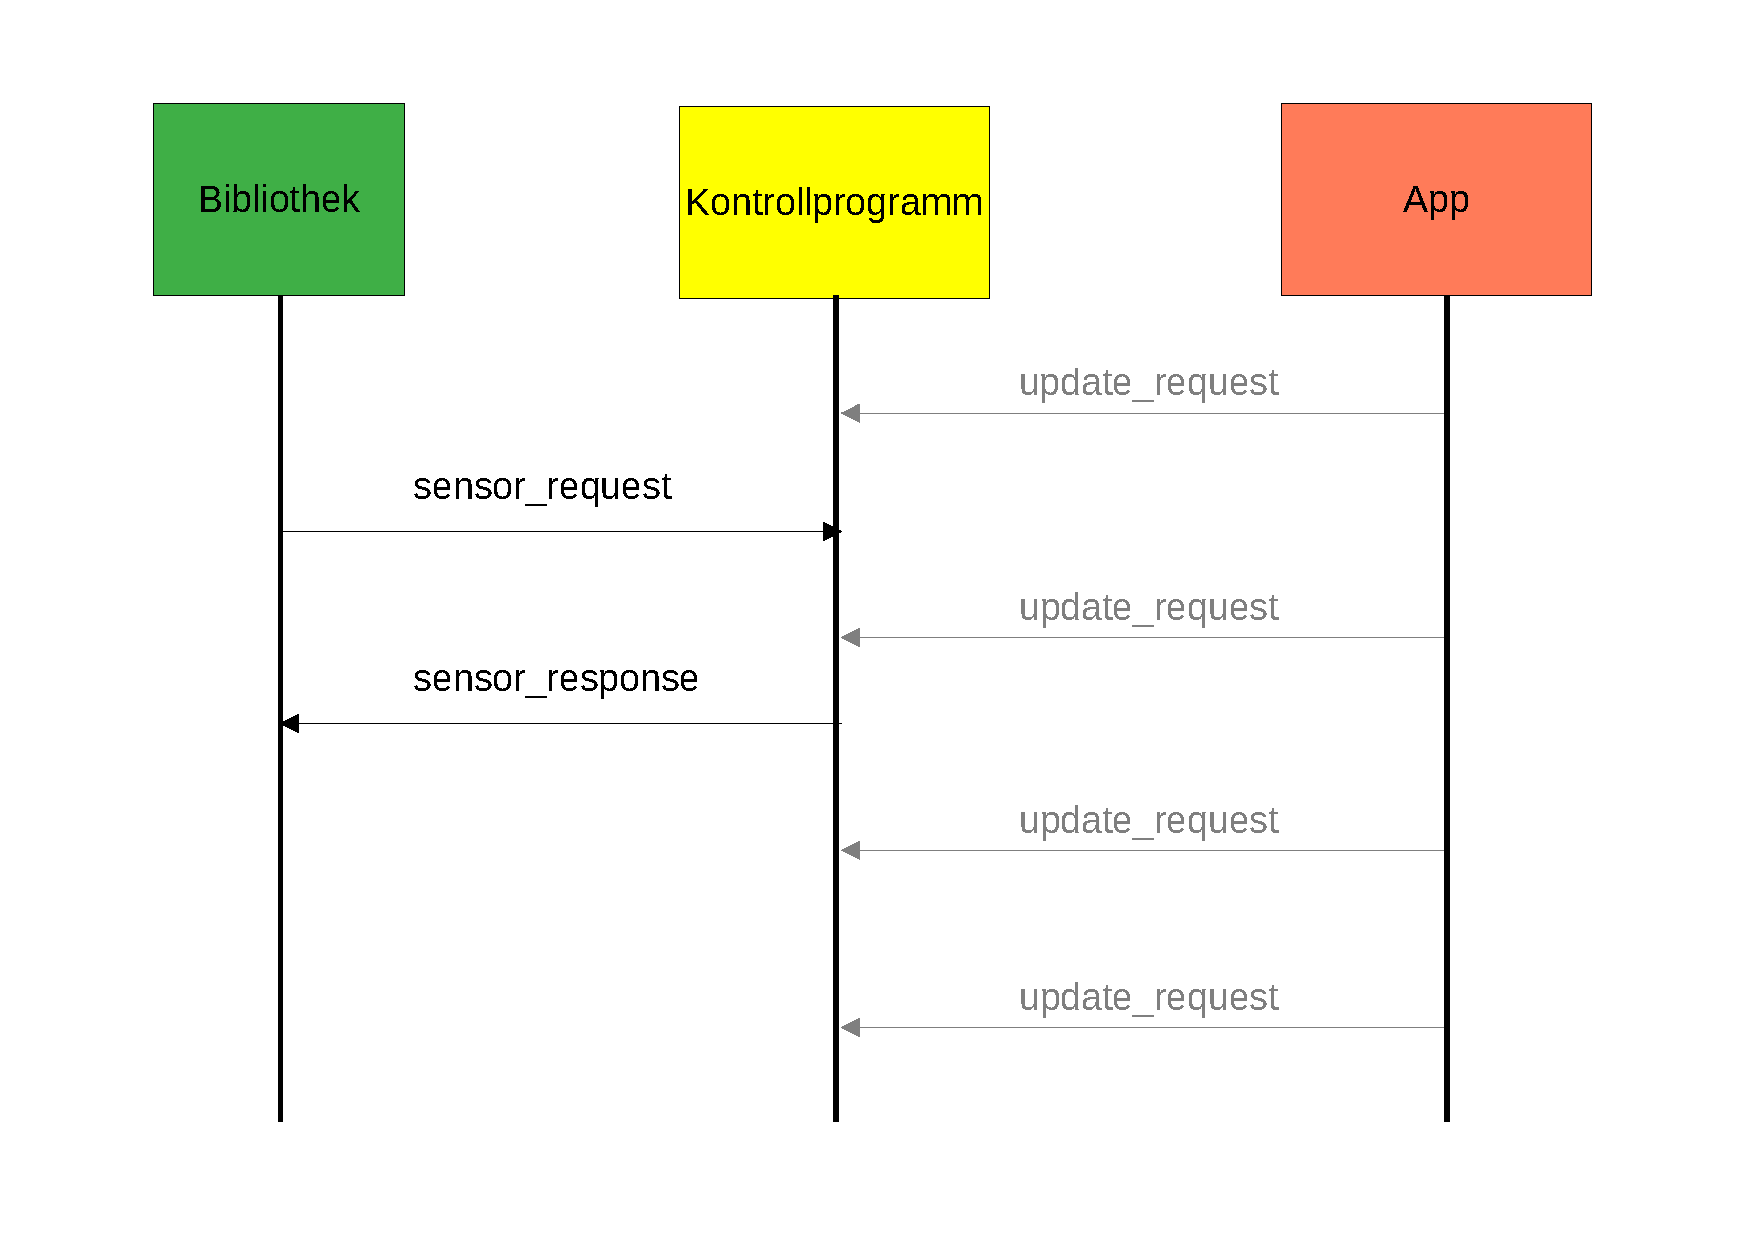
\includegraphics[width=.5\textwidth]{images/message_flow_sensor}
\caption{Nachrichtenablauf der Sensordatenübermittlung}
\label{fig:message_flow_requests}
\end{figure}
Aufgeführt sind die drei Komponenten Bibliothek, Kontrollprogramm und Smartphone-App.
Die Bibliothek sendet \texttt{sensor\_requests} per UDP an das Kontrollprogramm.
Dieses antwortet über UDP mit einer \texttt{sensor\_response}.
Währenddessen werden der Kontrollanwendung vom Smartphone fortwährend neue Sensormesswerte durch \texttt{update\_requests} übertragen.

Neben Nachrichten die die Sensordatenübermittlung betreffen, existieren zur Umsetzung von Ausgaben auf der Smartphone-App auch Ausgabe-Nachrichten.
Die app-seitigen Ausgaben sind unterscheidbar in Ausgaben mit und ohne Rückgabewert.
Für erstere gibt es den Nachrichtentyp \texttt{rpc\_request}.

\acrfull{rpc} bezeichnet clientseitige Funktionsaufrufe, die auf einem Server ausgeführt werden.
Die Bezeichnung entspricht nicht exakt dem Konzept, da ein Kommunikationspartner, Smartphone-App oder Kontrollanwendung, in diesem Fall die Rolle des Servers einnehmen würde.
Die Voraussetzung einer Client-Server-Anwendung ist durch die beidseitige Nachrichtenübertragung zwischen Smartphone-App und Kontrollanwendung nicht gegeben.
Die Bezeichnung wurde unter dem Fokus auf der entfernten Ausführung einer Funktion gewählt und entspricht eher einer \acrfull{rmi}.

Der Nachrichtentyp \texttt{rpc\_request} enthält die Felder \texttt{command} und \texttt{value}.
Diese spezifizieren die Ausgabe und falls vorgesehen eine mit der Ausgabe verbundene Größe.
Für die Vibrationsausgabe wären die Inhalte des \texttt{rpc\_requests} für eine Vibration von einer Sekunde beispielsweise \texttt{vibrate} und \texttt{1000}.
Die Nachricht wird von der Bibliothek per UDP an die Kontrollanwendung und von dort aus per MQTT an das Smartphone gesendet.
Die Smartphone-App nimmt die Anfrage an und führt die Ausgabe aus.
Manche Ausgabe-Anweisungen geben zusätzlich einen Rückgabewert zurück.
Damit dieser vom Smartphone zurück an die Bibliothek gesendet werden kann, gibt es das Nachrichtenformat \texttt{rpc\_response}.
Eine Nachricht dieser Nachrichtenart wird erst per MQTT an das Kontrollprogramm und von dort aus per UDP an die Bibliothek gesendet.
Der Nachrichtenablauf wird in Abbildung \ref{fig:message_flow_rpc} dargestellt.
\begin{figure}[htbp]
\centering
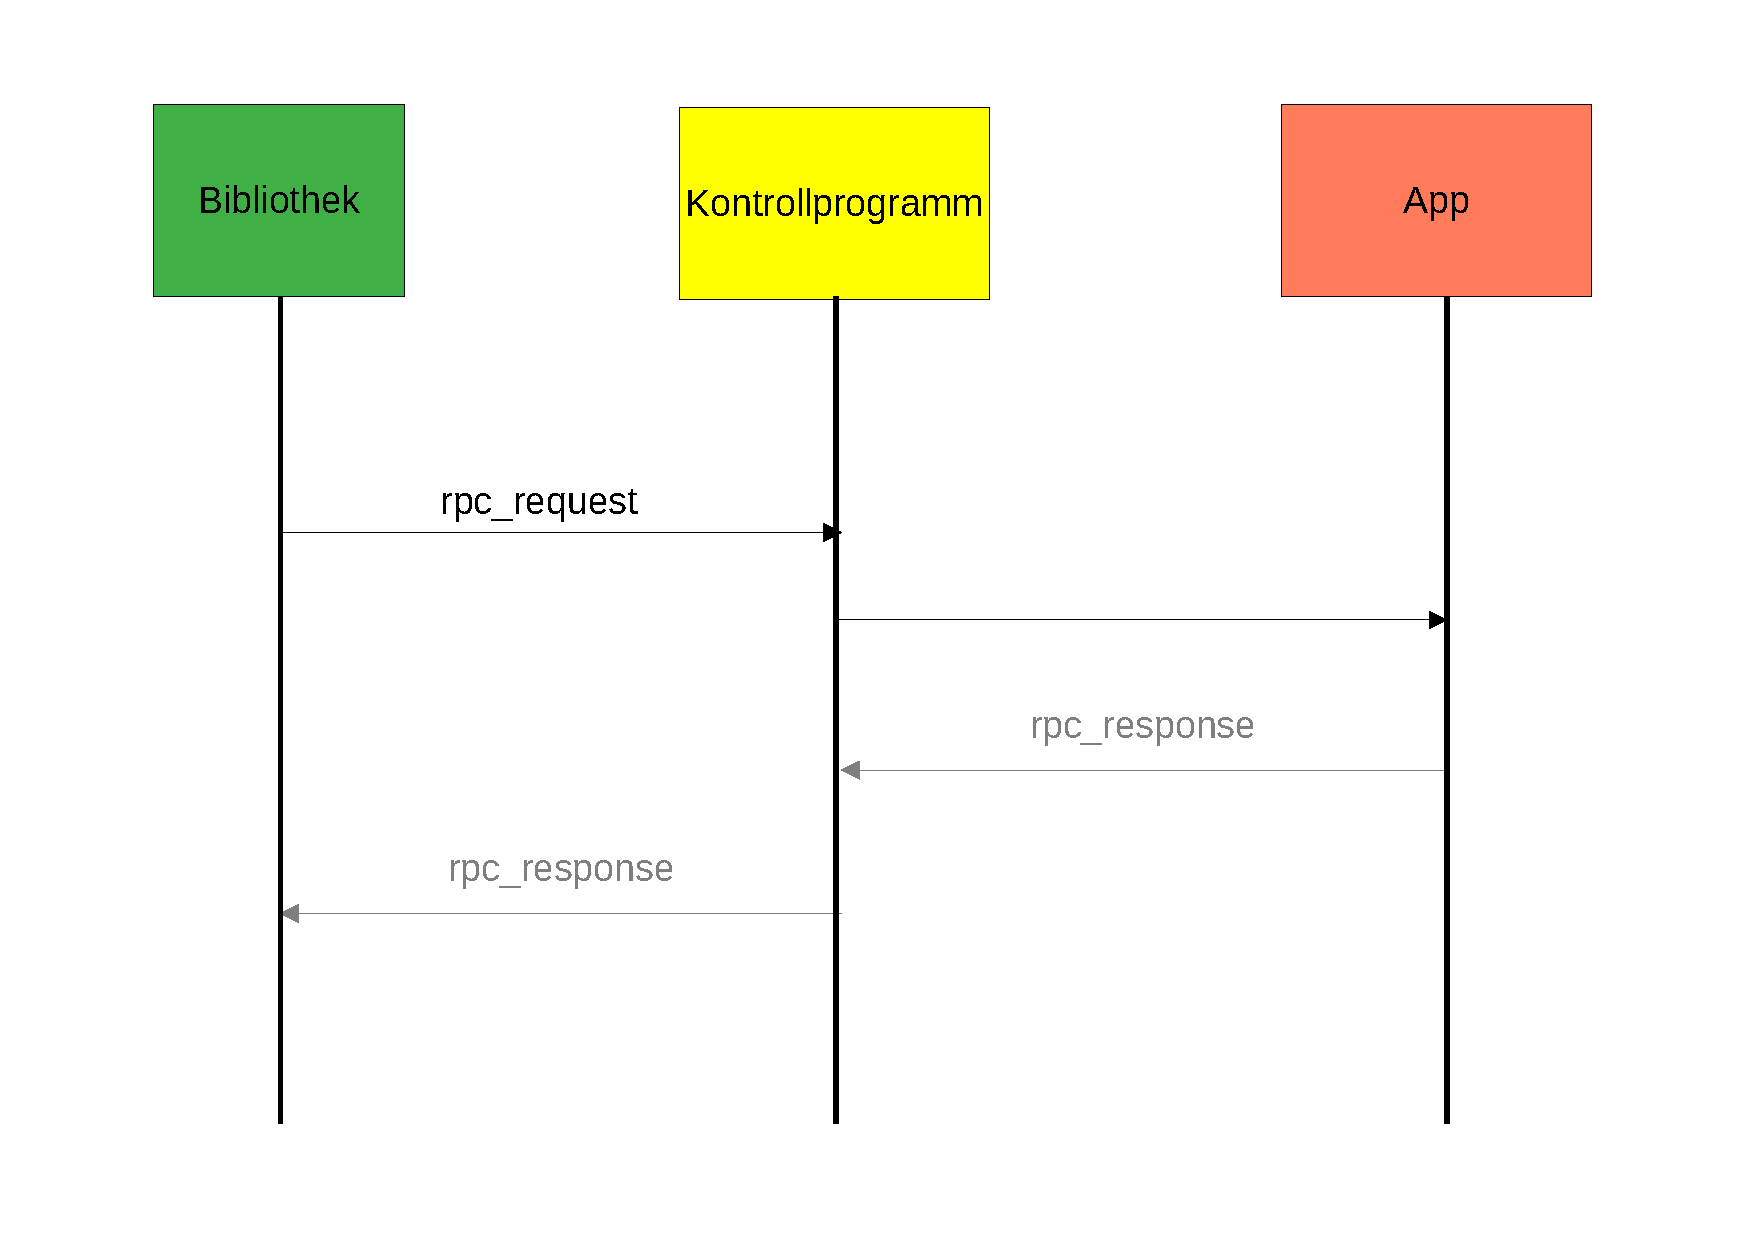
\includegraphics[width=.5\textwidth]{images/message_flow_rpc.pdf}
\caption{Nachrichtenablauf der RPC-Anfragen}
\label{fig:message_flow_rpc}
\end{figure}
Aufgeführt sind die drei Komponenten Bibliothek, Kontrollprogramm und Android-App.
Die Bibliothek sendet ein \texttt{rpc\_request} per UDP an das Kontrollprogramm.
Dieses leitet die Nachricht per MQTT weiter an die Smartphone-App, wo das Kommando ausgeführt wird.
Ein eventuell anfallender Rückgabewert wird durch eine \texttt{rpc\_response} vom Smartphone per MQTT zurück an die Kontrollanwendung gesendet, welche die Nachricht dann per UDP weiter an die Bibliothek weiterleitet.

\chapter{Aufbau der Programmierumgebung}\label{chap:libs}
Die Programmierumgebung ist die Schnittstelle, die die Programmierer für die Interaktion mit dem Smartphone in ihren Programmen verwenden.
Sie besteht aus einer Bibliothek, die Funktionen anbietet mit denen Programmierer Sensormesswerte des Smartphones einlesen, oder Ausgaben auf dem Smartphone tätigen können.
Sie können die Funktionen in ihren bestehenden Quellcode einbinden und die Funktionen dort verwenden.
In diesem Kapitel wird der Aufbau der Bibliothek und der Ablauf der angebotenen Funktionen beschrieben. 

Die Bibliothek existiert zur Kompatibilität für Programme der Programmiersprachen C, Java und Python.
In Java und Python ist sie zudem plattformunabhängig.
Für C gibt es zwei Bibliotheken: Eine für Unix- und eine für Windows-Systeme.
In C ist die Bibliothek prozedural mit statischen Methoden, in Java und Python objektorientiert implementiert.
%todo: Warum genau diese Programmiersprachen? Facts über Verteilung.

Werden die bereitgestellten Funktionen aufgerufen, werden standardisierte Anfragen im JSON-Format generiert und an die Kontrollanwendung gesendet.
Zur Verbesserung der Verständlichkeit für angehende Programmierer, wird auf Funktionen mit asynchronen Rückgabewerten, wie beispielsweise Futures, verzichtet.
Diese sendet die Daten gegebenenfalls an das Smartphone weiter oder antwortet direkt.
Eine Übersicht ist in Abbildung \ref{fig:Schnittstelle Bibliothek} dargestellt.
\begin{figure}[htbp]
  \centering
  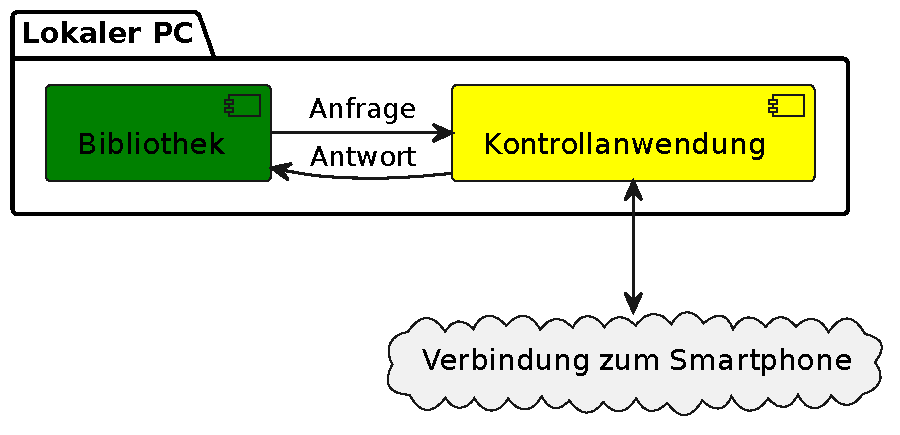
\includegraphics[width=.6\textwidth]{images/lib_server_connection}
  \caption{Schnittstellen der Bibliothek}
  \label{fig:Schnittstelle Bibliothek}
\end{figure}

Alle Anfragen werden über das UDP-Protokoll unter IPv4 versendet.
Das Kontrollprogramm ist auf dem Port 5006 erreichbar, Bibliotheken auf dem Port 5005.
Beide kommunizieren über die localhost-Adresse 127.0.0.1.
Dadurch werden Datagramme über das Loopback-Interface gesendet.
Zum Senden und Empfangen von Anfragen werden Sockets verwendet.
Für das Empfangen von Paketen müssen diese gebunden werden, für Sendevorgänge nicht.

Bei der Erstellung eines Phone-Objekts in Python und Java werden die Nachrichtenvorlagen für Anfragen und Antworten aus der Datei \texttt{protocol.json} geladen.
Die Datei muss sich im Dateisystem im gleichen Ordner befinden wie die Bibliothek.
Für die C-Bibliothek sind alle Methoden statisch definiert.
Es gibt somit keinen Startpunkt, zu dem die Datei \texttt{protocol.json} eingelesen werden kann.
Damit die Datei nicht für jeden Funktionsaufruf kontinuierlich eingelesen werden muss, muss ihr Inhalt von der Programmiererin oder dem Programmierer einmal zum Start des Programms als C-String eingelesen werden.
Anschließend muss dieser C-String für jeden Aufruf einer Funktion der Bibliothek als Parameter angegeben werden.
Die Methode \texttt{get\_file\_content} kann, unter der Angabe des Dateipfades der \textit{protocol.json}-Datei, aufgerufen werden, um den Dateiinhalt einzulesen und den Inhalt als C-String zurück zu erhalten.
Diese Lösung verringert die Anzahl der Lesevorgänge und die damit verbundenen, durch IO-Vorgänge verursachten, Latenzen.
Der Inhalt ist ab dem Einlesezeitpunkt auf dem Heap des Arbeitsspeichers gespeichert.
Der Programmierer muss diesen am Ende seines Programms durch den Aufruf der \texttt{free}-Funktion wieder freigeben.
%todo: Kapitel JSON Parser. Einbinden für die Kompilierung was woher beziehen usw.

\chapter{Aufbau der Kontrollanwendung}\label{chap:server_software}
Zur Vermittlung zwischen der Smartphone-App und Programmierumgebung dient die Kontrollanwendung.
Die Anwendung vermittelt als Middleware zwischen Anfragen der Programmierumgebung und Anfragen der mobilen Anwendung.
Durch Sie können Ausgaben in der Android-App ausgeführt- und Sensordaten abgefragt werden.
Sie wurde in Python entwickelt und ist aus mehreren Komponenten aufgebaut.
In diesem Kapitel wird der Aufbau der Anwendung anhand ihrer zweckgebundenen Komponenten dargestellt und die Funktionsweise der Bestandteile im Detail an Beispielen erläutert.

Die Kontrollanwendung besteht aus mehreren Thread-Klassen, die beim Start der Anwendung gestartet werden.
Sie ist mit den Klassen DataHandler und MQTTHandlerThread aufgeteilt in einen Daten verwaltenden Bestandteil und eine MQTT-Anbindung.
Zusätzlich dient eine Instanz der Klasse SensorDB als Key-Value-Store um die vom Smartphone übermittelten Sensordaten zwischenzuspeichern.
SensorDB bietet einen threadsicheren Zugriff auf ein intern gespeichertes Python-Dictionary.
Eine Übersicht über die Komponenten der Kontrollanwendung ist in Abbildung \ref{fig:serverUml} dargestellt.
\begin{figure}[htbp]
  \centering
  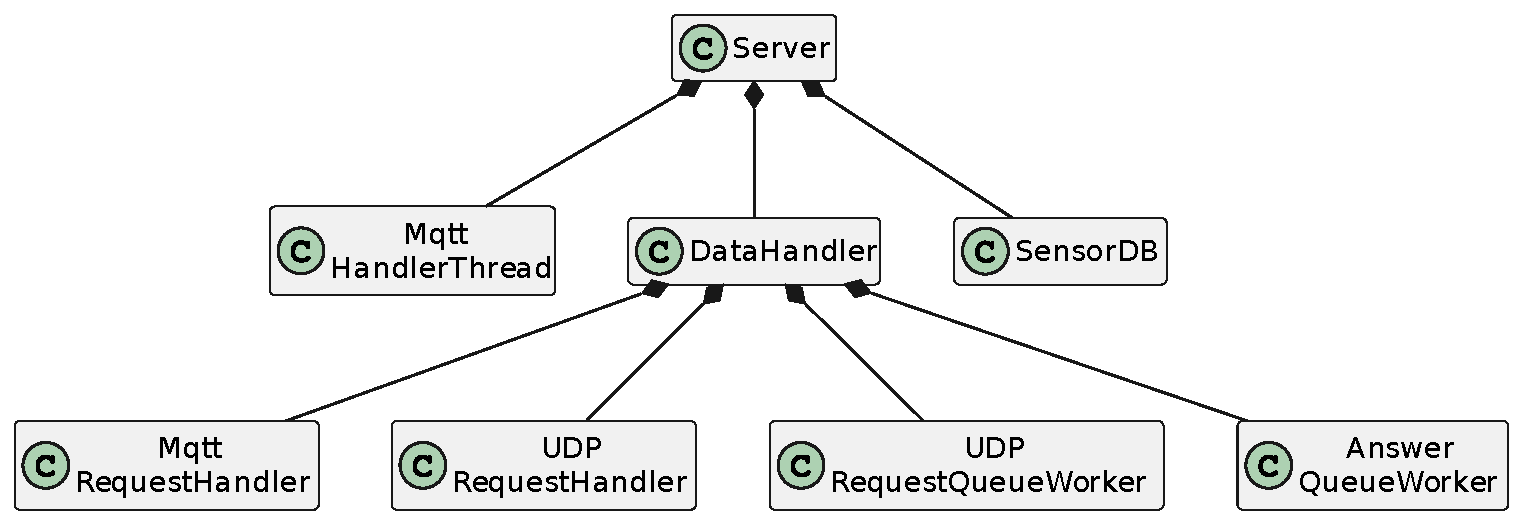
\includegraphics[width=\textwidth]{images/ServerUml}
  \caption{UML Digaramm Server}
  \label{fig:serverUml}
\end{figure}

Die Komponente DataHandler besteht wiederum aus vier Sub-Komponenten, die ebenfalls als Threads nebenläufig laufen: MqttRequestHandler, UDPRequestHandler, UDPRequestQueueWorker und AnswerQueueWorker.
Ziel der Aufteilung der Arbeitsschritte in Threads ist die Gewährleistung der Verfügbarkeit für beide Kommunikationspartner.
Die Thread-Kommunikation wird durch die threadsichere Fifo-Datenstruktur queues \cite{python_queue} realisiert.
Nachrichten werden von einem Thread in der queue abgelegt und in einem anderen aus der queue entnommen.
Eine durch das polling verursachte hohe CPU-Last kann durch blockierende Operationen beim ablegen und herausnehmen abgewendet werden.

Die Funktionsweise und Zwecke der Subkomponenten von DataHandler werden im Folgenden anhand zweier Beispiele erläutert.
Abbildung \ref{fig:serverMqttReqPath} wird zur Erläuterung für das erste Beispiel diskutiert.
\begin{figure}[htbp]
  \centering
  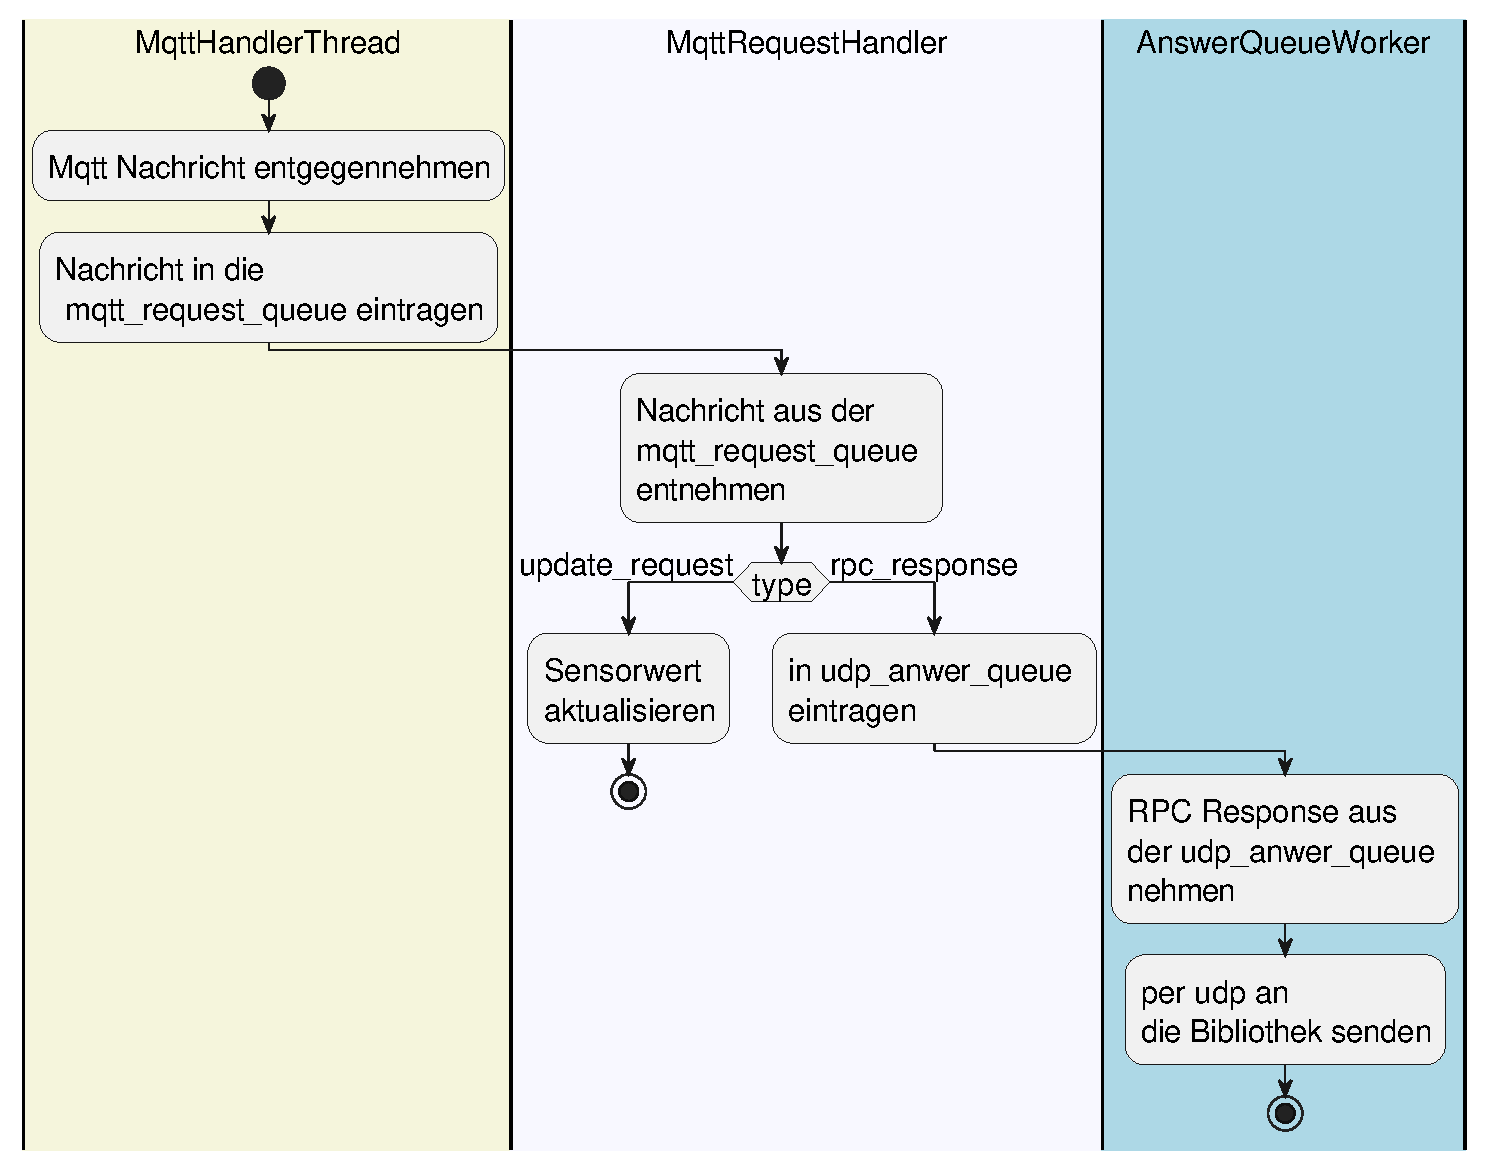
\includegraphics[width=\textwidth]{images/MqttRequestServerPath}
  \caption{Ablaufdiagramm MQTT Request}
  \label{fig:serverMqttReqPath}
\end{figure}
Dargestellt ist der Ablaufplan bei Empfang einer von der mobilen Anwendung an die Kontrollanwendung per MQTT versandten Nachricht.
Dies könnte beispielsweise ein \texttt{update\_request} sein.

Für die MQTT-Verbindung wird die unter OpenSource-Lizenz stehende MQTT-Library Paho \cite{paho} der Eclipse-Foundation verwendet. 
Erreicht eine Nachricht per MQTT die Anwendung, wird Sie vom MQTTHandlerThread entgegengenommen.
Dieser hat sich mit einem MQTT-Broker unter der Hostadresse \textit{pma.inftech.hs-mannheim.de} auf ein in der Datei \textit{config.json} angegebenes Topic verbunden und reagiert mit einer Callback-Methode auf eingehende Nachrichten.
Erreicht eine Nachricht den MQTTHandlerThread, wird die Callback-Funktion ausgelöst und die Payload der Nachricht in eine Queue eingetragen.
Der MqttRequestHandler wartet, bis ein Eintrag in der Queue vorhanden ist, entnimmt gegebenenfalls eine Nachricht und bestimmt den Nachrichtentyp der Anfrage.
Prinzipiell können von der Smartphone-App nur zwei Nachrichtentypen an die Kontrollanwendung versandt werden.
Handelt sich um ein \texttt{update\_request}, also einen neuen Sensorwert, muss dieser in der Datenbank aktualisiert werden.
Handelt es sich hingegen um eine \texttt{rpc\_response}, also um eine Antwort auf eine vorausgegangenes \texttt{rpc\_request}, muss diese Nachricht per UDP an die Bibliothek zurückgesendet werden, wofür Sie in eine andere queue abgelegt wird.
Der AnswerQueueWorker wartet, bis der MqttRequestHandler die Nachricht abgelegt hat und sendet diese dann per UDP über die localhost-Adresse \textit{127.0.0.1} auf dem Port \textit{5005} zurück an die Bibliothek.

Das zweite Beispiel befasst sich mit dem Ablauf eines UDP-Requests, also einer mit UDP versandten Nachricht der Programmierumgebung.
Der Ablauf ist in Abbildung \ref{fig:serverUDPReqPath} dargestellt.
\begin{figure}[htbp]
  \centering
  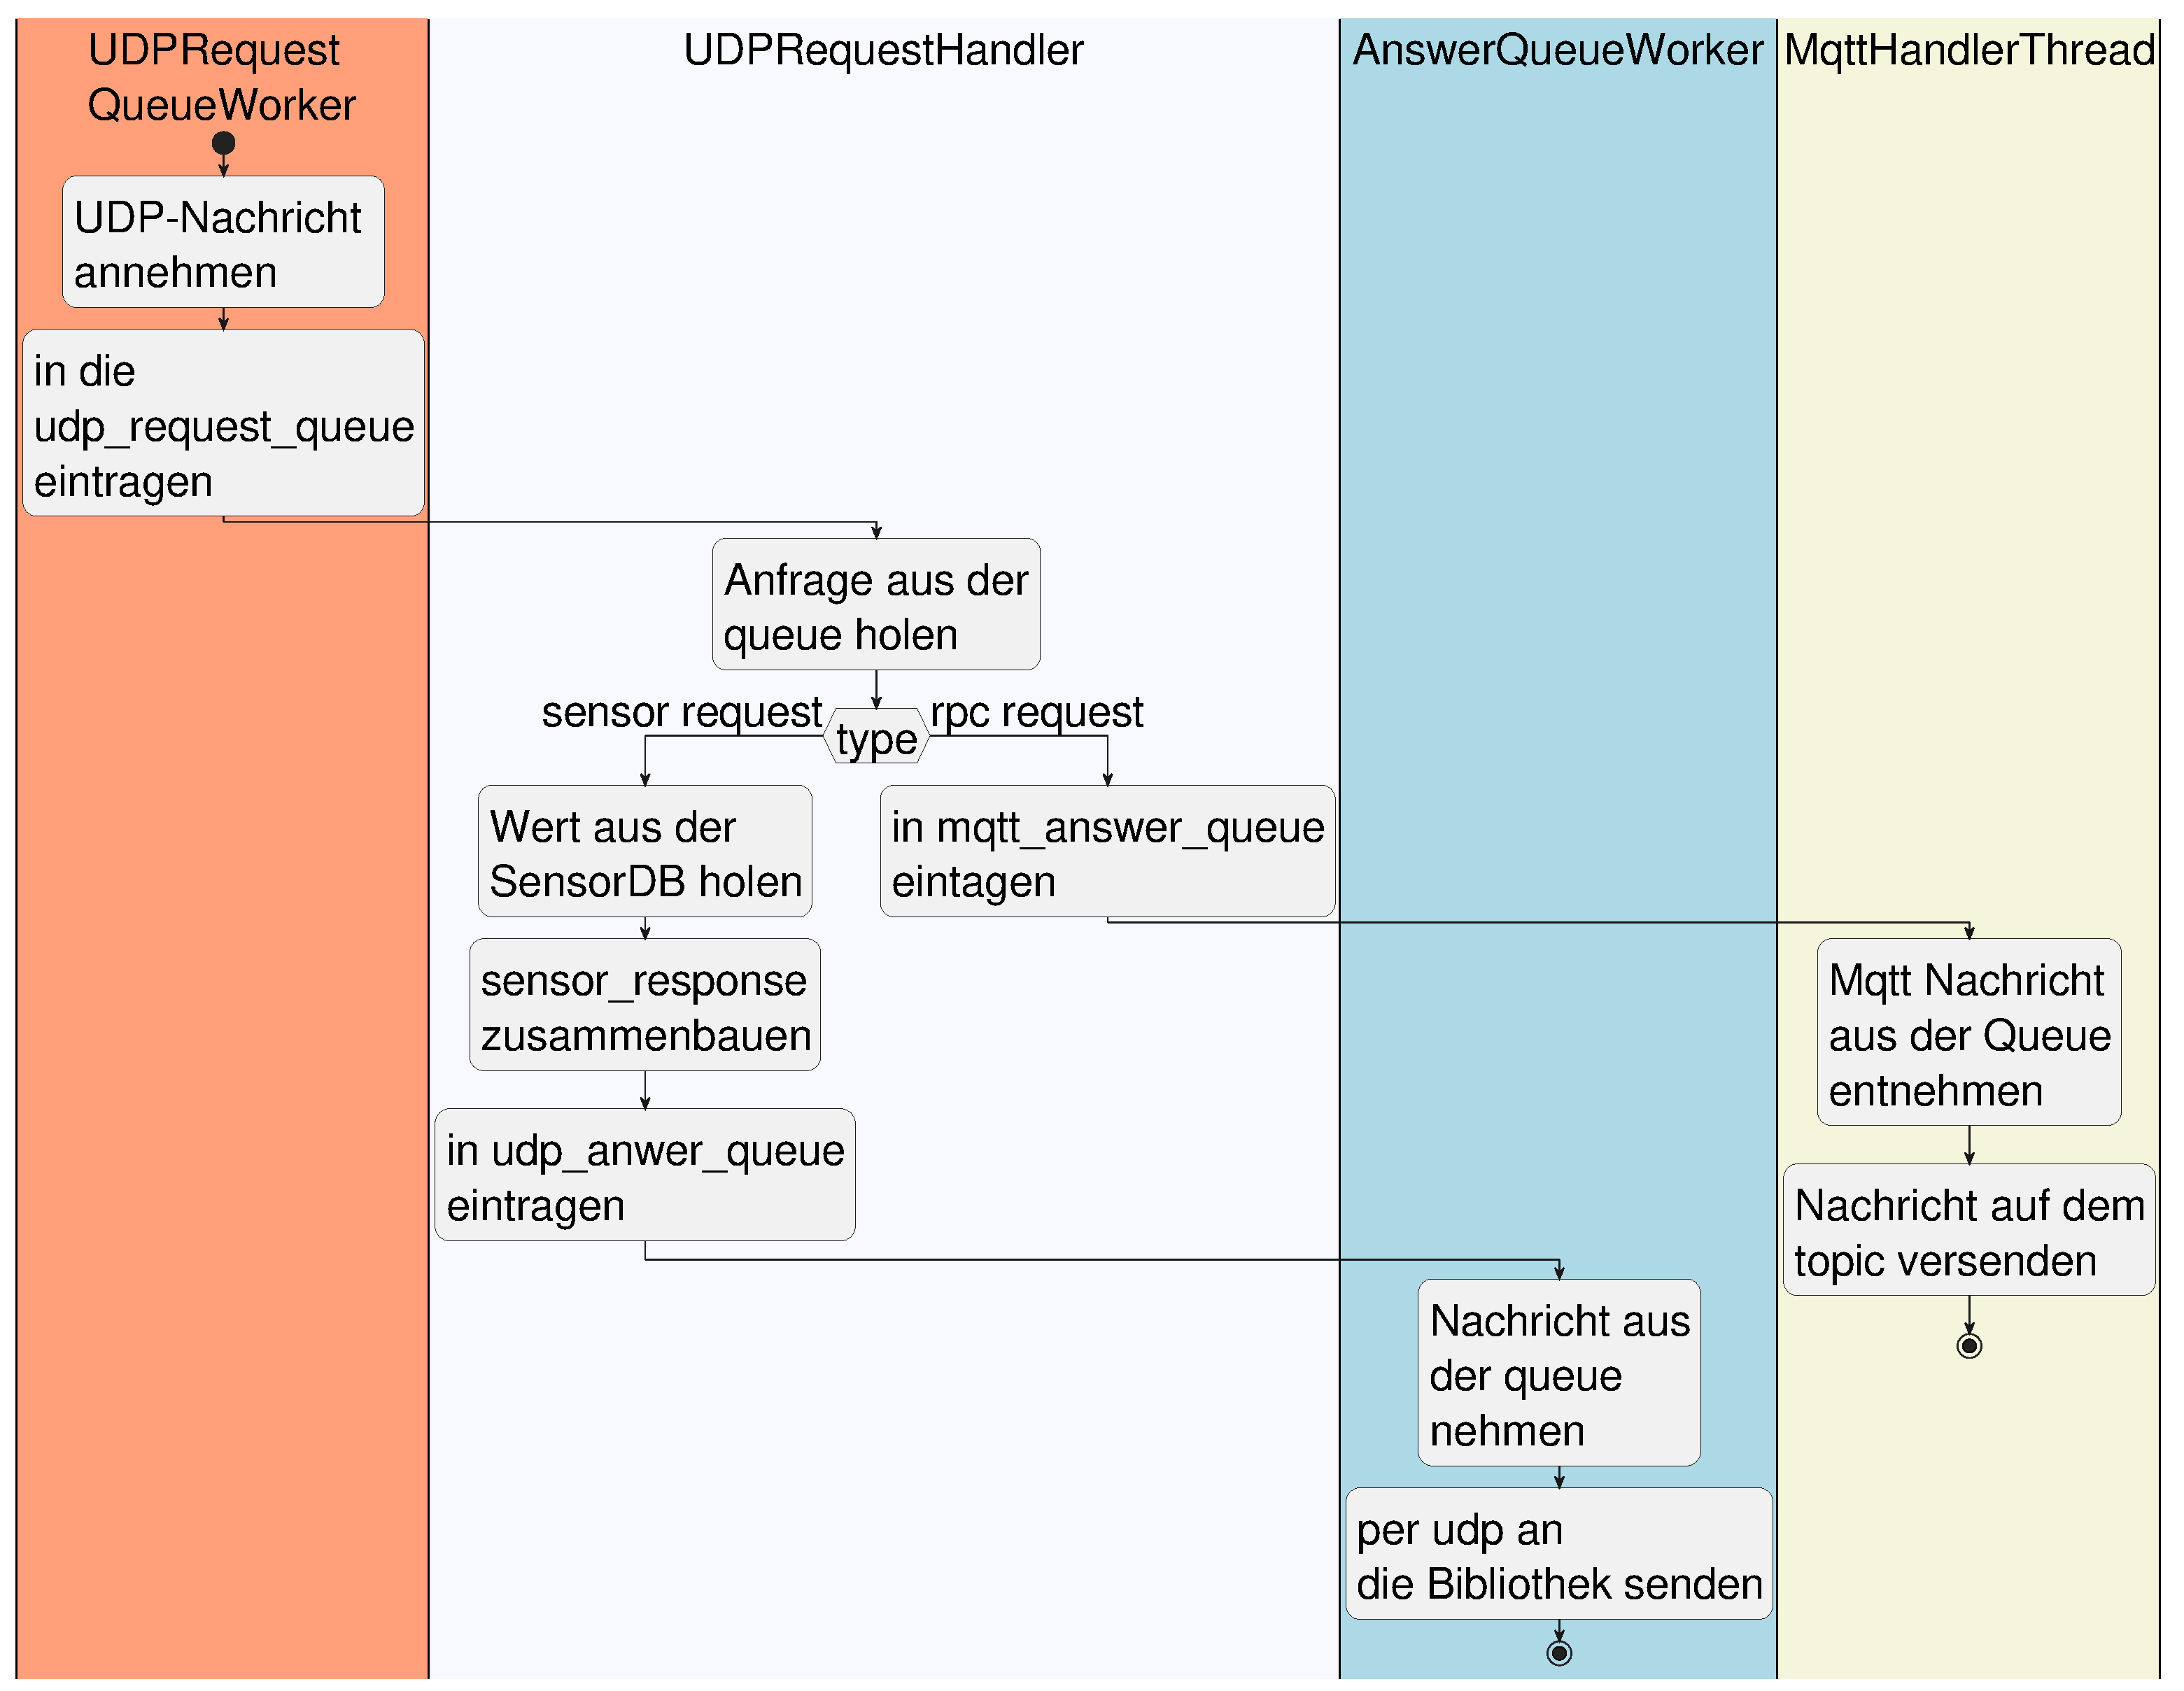
\includegraphics[width=\textwidth]{images/UDPRequestServerPath}
  \caption{Ablaufdiagramm UDP Request}
  \label{fig:serverUDPReqPath}
\end{figure}
Erreicht eine Nachricht per UDP die Anwendung, wird Sie vom UDPRequestQueueWorker entgegengenommen
Dieser bindet beim Start einen Socket für die localhost-Adresse \textit{127.0.0.1} und den Port \textit{5005}  ein.
Geht auf dem Socket eine Nachricht ein, wird Sie in eine queue abgelegt.
Der UDPRequestHandler entnimmt die Nachricht aus der queue und bestimmt den Typ der Anfrage.
Handelt es sich um eine Nachricht des Types \texttt{rpc\_request}, also einer Ausgabe-Anfrage für das Smartphone muss Sie per MQTT an das Smartphone versandt werden, wofür Sie in eine andere queue eingetragen wird.
Der MQTTHandlerThread entnimmt die Nachricht und sendet sie per MQTT ab.
Ist Nachricht hingegen ein \texttt{sensor\_request}, also die Anfrage eines Sensormesswerts, muss eine Nachricht des Typs \texttt{sensor\_response} erstellt und der ausgelesene Wert eingefügt werden.
Dieser wird unter Verwendung der SensorDB-Klasse ermittelt.
Die erstellte, befüllte Antwort muss anschließend an die Programmierumgebung zurückgesendet werden.
Hierfür wird die Anfrage vom UDPRequestHandler in eine Queue eingetragen, aus der der AnswerQueueWorker Sie wieder entnimmt und Sie an die Programmierumgebung zurücksendet.

Zusammenfassend erfüllen die Komponenten folgende Aufgaben.
Der MQTTHandlerThread nimmt Nachrichten per MQTT an und sendet Sie ab.
Das Gegenstück dazu bilden für UDP-Anfragen der UDPRequestQueueWorker, der Anfragen von der Programmierumgebung annimmt und der AnswerQueueWorker, der Anfragen an diese zurücksendet.
Aufgabe des des MqttRequestHandler ist die Bearbeitung von MQTT Requests.

\chapter{Aufbau der Android-Anwendung}\label{chap:app}
Die Android-Anwendung ist eine der drei Bestandteile des Frameworks.
Sie dient dazu Sensormessprozesse zu starten, Sensordaten zu übermitteln und Ausgabe-Kommandos auszuführen.
Der Aufbau und die internen Abläufe in Bezug auf Nachrichtenempfang auf automatisierter Übertragung der Sensormesswerte werden in diesem Kapitel im Detail beschrieben.

Als visuelle Ausgabemöglichkeiten bietet die Android-Anwendung eine Signal-LED, ein Textfeld und zwei Buttons in einer RootActivity an.
Neben UI-Elementen gibt es zusätzlich noch eine Vibrationsausgabe. 
Die Anwendung initiiert zum Start Sensormessprozesse und sendet unter Verwendung von SensorEventListenern die Sensormessdaten in periodischen Zeitabständen an die Kontrollanwendung.
Zur Verwendung kommende Sensortypen sind beispielsweise der Lagesensor oder das Gyroskop des Smartphones.
Die gemessenen Werte werden über einen im Hintergrund ausgeführten MQTT-Service versandt, welcher ebenfalls auf eingehende Nachrichten reagiert, um Ausgaben auf dem Smartphone auszulösen.

\section{Startvorgang}
Ein Ablaufplan des Startvorgangs ist in Abbildung \ref{fig:app_flow} dargestellt.
\begin{figure}[htbp]
  \centering
  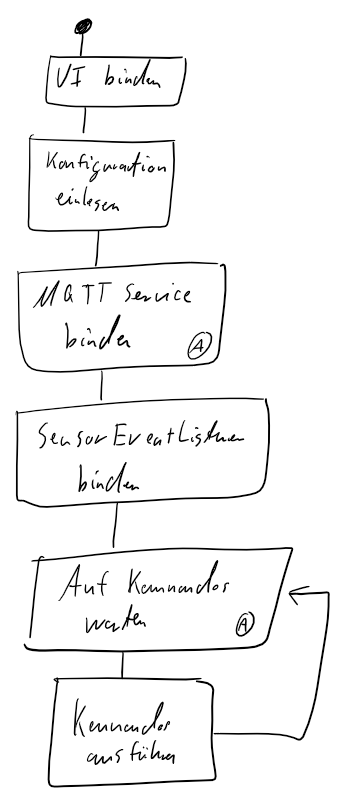
\includegraphics[width=0.8\textwidth]{images/app_ablauf}
  \caption{Ablaufdiagramm Android-Anwendung}
  \label{fig:app_flow}
\end{figure}
In der RootActivity werden anfänglich alle UI-Elemente zur programmatischen Ansteuerung eingebunden.
Anschließend werden die zwei Konfigurationsdaten config.json und protocol.json eingelesen.
In Ersterer sind grundlegende Konfigurationsparameter wie Hostname und Port des MQTT-Brokers oder der Name des Topics definiert.
In der Datei protocol.json werden neben den Schlüsselwörtern und Abkürzungen für Sensortypen und Ausgabekommandos auch Vorlagen für Nachrichtenformate aufgeführt.

Nach dem Einlesen der Konfigurationen wird der zur Kommunikation verwendete MQTT-Service gestartet und asynchron eingebunden.
Über eine ServiceConnection wird beim erfolgreichen Einbinden über eine Callback-Methode der weitere Ablauf der Anwendung definiert, der erst ausgeführt werden soll, wenn eine MQTT-Verbindung hergestellt ist.
RootActivity und MQTT-Service tauschen jeweils ihre Objekt-Referenzen aus.
Methoden des MQTT-Service rufen zum Zweck der Ausgabe Methoden der RootActivity auf.
SensorEventListener benötigen eine Referenz auf den MQTT-Service, da sie bei Sensorwerten über diesen \texttt{update\_request}s versenden.

Der Nachrichtenempfang im MQTT-Service wird nicht im UI-Thread behandelt.
Dies ist jedoch Voraussetzung um UI-Elemente wie zum Beispiel die Farbe der Signal-LED im Service verändern zu können.
Android unterbindet Änderungen aus Threads getätigt werden nicht, UI-Thread sind.
Dieses Problem wird durch die Methode \textit{runOnUiThread} umgangen, welche die Änderung in der Ausführungswarteschlange des UI-Threads einreiht.
Eine Übersicht des Vorgangs in in Abbildung \ref{fig:runOnUiThread} dargestellt.
\begin{figure}[htbp]
  \centering
  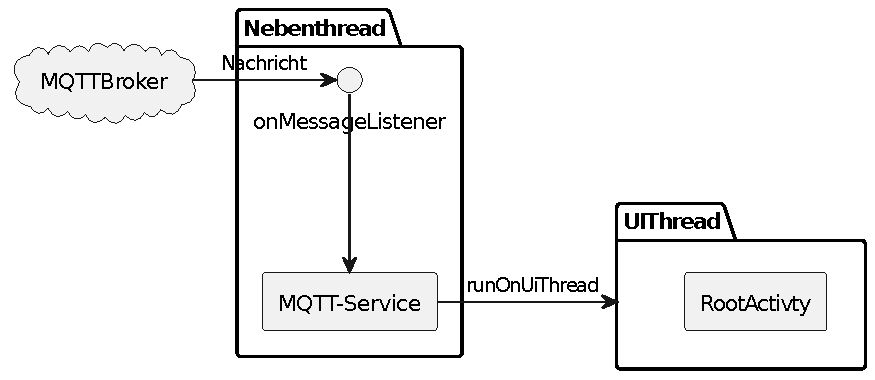
\includegraphics[width=0.8\textwidth]{images/runOnUiThread.pdf}
  \caption{Ausführung auf dem UI-Thread}
  \label{fig:runOnUiThread}
\end{figure}

Der MQTT-Service baut eine Verbindung zu einem in Datei config.json definierten MQTT-Broker auf und abonniert ein ebenfalls in der Konfigurationsdatei angegebenes Topic.
Ist der MQTT-Service eingebunden sind alle Voraussetzungen für eine Übertragung erfüllt und  Sensormessprozesse können gestartet werden.
Die Funktionsweise der Sensormessung wird in Abbildung \ref{fig:sensor_event_listener} dargestellt.
\begin{figure}[htbp]
  \centering
  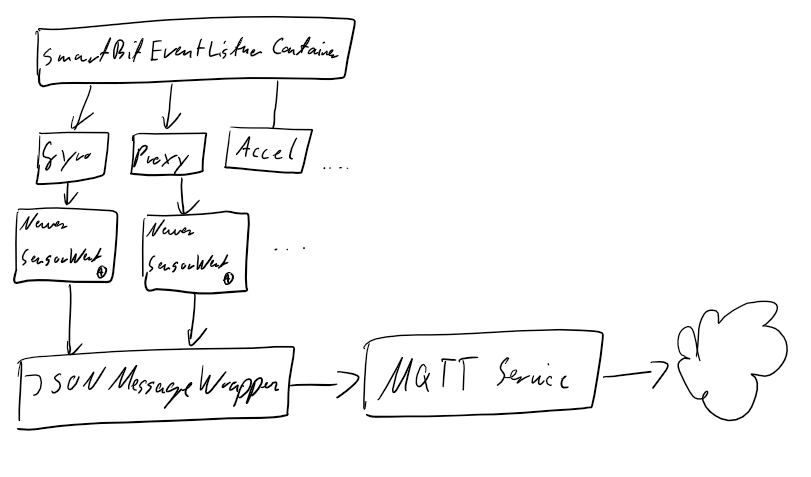
\includegraphics[width=.8\textwidth]{images/sensor_event_listener}
  \caption{Ablauf SensorEventListener}
  \label{fig:sensor_event_listener}
\end{figure}
SensorEventListener werden, nach Prüfung der Verfügbarkeit der jeweiligen Sensoren, gestartet und zentral in der Instanz der Klasse \texttt{SmartBitEventListenerContainer} gespeichert.
Diese Klasse beinhaltet SensorEventListener für alle unterstützten Sensoren und dient ihrer Datenhaltung.
Aufgabe der SensorEventListener ist es, auf Sensorwert-Änderungen zu reagieren und gegebenenfalls die Callback-Funktion \texttt{onSensorChanged()} auszuführen, in der die Sensorwerte über den MQTT-Service per \texttt{update\_requests} an die Kontrollanwendung übermittelt werden.
Statische Methoden der Klasse \textit{JSONMessageWrapper} ermöglichen die Erstellung der Nachrichtenformate und setzen das Messergebnis in das entsprechende Feld in der JSON-Nachricht ein.
Die so generierte Nachricht wird anschließend über den gebundenen MQTT-Service an das vorher definierte Topic versandt.

Ist der Erhalt von Nachrichten möglich und werden Sensormessdaten automatisch an die Kontrollanwendung gesendet, ist die Startroutine der mobilen Anwendung abgeschlossen.
Auf Nachrichten wird nun nur noch im MQTT-Service in einem MessageListener mit entsprechendem Callback reagiert und gegebenenfalls eine Ausgabe ausgeführt.
Die Anwendung ist nun betriebsbereit und sendet \texttt{update\_request}s an die Kontrollanwendung.
Übermittelt werden die Sensordaten an den Broker mit einer \acrfull{qos} (Quality of Service) von 0.
Auf dieser Stufe wird der Empfang der Nachricht von den Kommunikationspartnern nicht bestätigt.
Verluste von \texttt{update\_request}s sind unproblematisch, da je nach Taktung der SensorEventListener innerhalb kurzer Zeit neue Sensormesswerte zur Übertragung vorliegen.
Eine exakte Zustellung ist hier nicht notwendig.
Höhere QoS-Stufen würden den Übertragungsprozess verlangsamen und Latenzen erhöhen.

\section{Sensoren}
Smartphones beinhalten Sensoren, die Daten über die Umgebungseigenschaften erfassen.
Dazu zählen beispielsweise Bewegung, Annäherung, aber auch Temperatur oder Luftdruck.
%todo: stimmt nicht. die messen einfach. reagiert wird wo anders.
Ihr Zweck besteht darin, auf Änderungen der Werte zu reagieren.
Für unterschiedliche Aufgaben werden unterschiedliche Sensoren benötigt.
Beispielsweise word für \textit{Diebstahl-Alarm} nur der Näherungssensor verwendet, für \textit{Dreh-Zähler} der Lagesensor.
Für die in dieser Arbeit enthaltenen Übungsaufgaben werden folgende Sensortypen verwendet: Beschleunigungssensor, Gyroskop und Annäherungssensor.

Beschleunigungs- bzw. Lagesensoren messen die Beschleunigung in $m/s^2$ für die drei Bewegungsrichtungen: X-, Y- und Z-Achse in einem festgelegten Zeitraum.
Zur Übersicht sind diese in Abbildung \ref{fig:and_axes} dargestellt.
\begin{figure}[htbp]
  \centering
  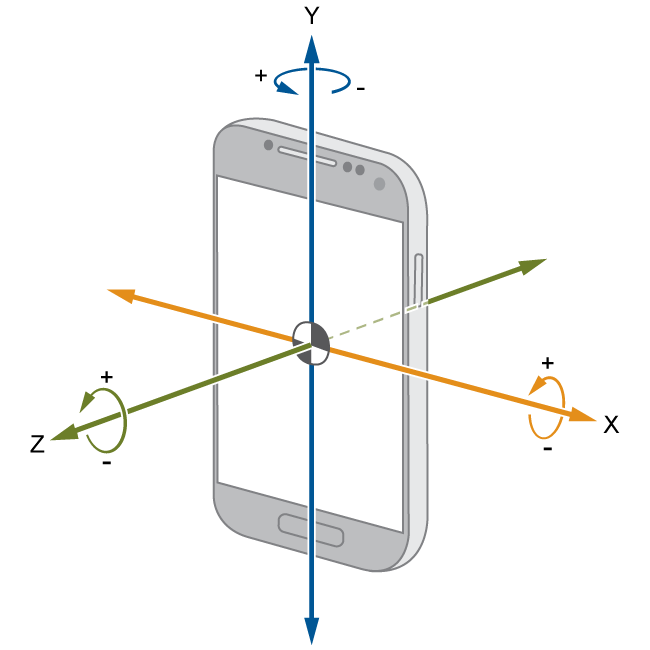
\includegraphics[width=.7\textwidth]{images/android_axes.png}
  \caption{Android-Koordinatensystem}
  \label{fig:and_axes}
\end{figure}
Die Erdbeschleunigung ist auch in diesen Messwerten enthalten.
Diese muss für die bereinigten, realen Werte von den aufgenommenen Werten subtrahiert werden\cite{accel_g}.
% todo: einheiten
Messeinheiten unterscheiden sich je nach Sensor.
Das Gyroskop misst keine Beschleunigung, sondern die aktuelle Geschwindigkeit in $rad/s$ der gleichen Achsen.

Die Frequenz, mit der Messwerte erfasst werden kann manuell angegeben werden.
Hierfür stehen vier Stufen zur Auswahl.
\begin{table}[htbp]
  \centering
  \begin{tabular}{|c|p{4cm}|}
      \hline
      \textbf{Bezeichnung} & \textbf{Maximale Verzögerung} \\
	  \hline
      SENSOR\_DELAY\_FASTEST & Keine. Verwendet die Frequenz des Sensors.\\
      \hline
      SENSOR\_DELAY\_GAME & 20 ms\\
      \hline
      SENSOR\_DELAY\_UI & 60 ms\\
      \hline
      SENSOR\_DELAY\_NORMAL & 200 ms\\
      \hline
  \end{tabular}
  \caption{Sensor-Taktgeschwindigkeiten\cite{sensor-takt}}
  \label{tab:sensor_speeds}
\end{table}
In der Android-App erfolgen alle Messungen mit SENSOR\_DELAY\_NORMAL.
Die Stufe gilt für Android jedoch nicht als festes Limit, sondern wird eher als Richt-Frequenz behandelt.
Android kann die reale Frequenz auch erhöhen.
Nicht alle Smartphones besitzen alle Sensoren.
Daher wird beim Start überprüft, ob der Sensor auch wirklich vorhanden ist.
Ist er es nicht, wird auch keine Messung gestartet.

\chapter{Evaluation der Smartbit-Lösung}\label{chap:eval}
Die Umsetzung der an die implementierte Anwendung gestellten Anforderungen wird in diesem Kapitel überprüft.
Durch Betrachtung eines Verwendungsbeispiels werden die Anforderungen qualitativ untersucht und anschließend bewertet.
Geringen Latenzzeiten wurden in der Konzeptionsphase eine hohe Priorität zugeordnet.
Diese werden anhand der Smartbit-Lösung für drei Nutzungsszenarien gemessen und bewertet.

\section{Verwendungsbeispiel}
Die Verwendung der Smartbit-Lösung wird anhand der Beispielaufgabe \textit{Alarmanlage} vorgestellt.
Gezeigt wird wie die Aufgabe in der Programmierumgebung unter Verwendung der Python-Bibliothek gelöst wurde und wie sich Ausgaben auf dem Smartphone äußern.
Die Android-Anwendung dieses Beispiels wurde auf den Smartphones Motorola G6 (Android 9), OnePlus 3T (Android 11) und Google Pixel 4 (Android 12) getestet.

Eine gestartete Kontrollanwendung ist Voraussetzung für einen Nachrichtenaustausch.
Mit dem Befehl \texttt{python ./server.py} wird sie in einer Shell gestartet.
Der Vorgang wird in Abbildung \ref{fig:start_controll_app} dargestellt.
\begin{figure}[htbp]
  \centering
  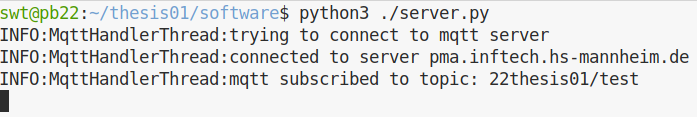
\includegraphics[width=.8\textwidth]{images/server_logging}
  \caption{Start der Kontrollanwendung}
  \label{fig:start_controll_app}
\end{figure}
Die Anwendung meldet eine erfolgreiche Verbindung mit dem MQTT-Broker und gibt das abonnierte Topic aus.
Neben diesen Start-Informationen werden auch eingehende \texttt{rpc\_requests} und \texttt{rpc\_responses} ausgegeben.
\texttt{sensor\_requests}, \texttt{sensor\_responses} und \texttt{update\_requests} werden wegen ihrer Häufigkeit nicht geloggt.

Die Implementierung der Lösung der Aufgabe ist in Listing \ref{lis:alarm} dargestellt.
\lstset{language=python, captionpos=b, frame=single, numberstyle=\tiny, style=customcs}
\lstinputlisting[label=lis:alarm, caption=Alarmanlage-Beispiel]{listings/code_examples/alarm.py}
Die Bibliothek wird in Zeile 2 in das vom Programmierer geschriebene Programm importiert, wofür sich die Datei \texttt{smartbit.py} und das entwickelte Programm im gleichen Ordner befinden müssen.
In Zeile 4 wird ein Phone-Objekt erstellt, über welches Sensor-Auslesemethoden wie \texttt{get\_x\_accel()} oder Smartphone-Ausgaben wie \texttt{vibrate()} aufgerufen werden können.
Das Programm soll nur im Falle eines KeyboardInterrupts angehalten werden.
In einer Endlosschleife wird der Näherungssensorwert kontinuierlich abgefragt.
Zusätzlich wird der Ablauf für 500 ms pausiert um einer Nachrichtenflut und somit einer Nichtverfügbarkeit der Kontrollanwendung vorzubeugen.
Der Annäherungssensor sendet im Falle einer Annäherung den Wert 0.0 zurück auf den in Zeile 8 reagiert wird.
Ist die Bedingung erfüllt, wird mit der Methode \texttt{write\_text()} der Text \textit{ALARM} ausgegeben.
Die Methode \textit{vibrate} lässt das Smartphone für die Dauer von 1000 ms vibrieren.
Zum Schluss wird mit der Methode \textit{toggle\_led} noch der Farbwert der Signal-LED von grün auf rot geändert.

Die Bibliothek übermittelt für jede Ausgabe korrespondierende \texttt{rpc\_requests} über die Kontrollanwendung an das Smartphone.
Bei Empfang werden die Anfragen in der Kontrollanwendung geloggt.
Eine Übersicht der gesendeten Nachrichten des Beispiels ist in Abbildung \ref{fig:req_controll_app} aufgeführt.
\begin{figure}[htbp]
  \centering
  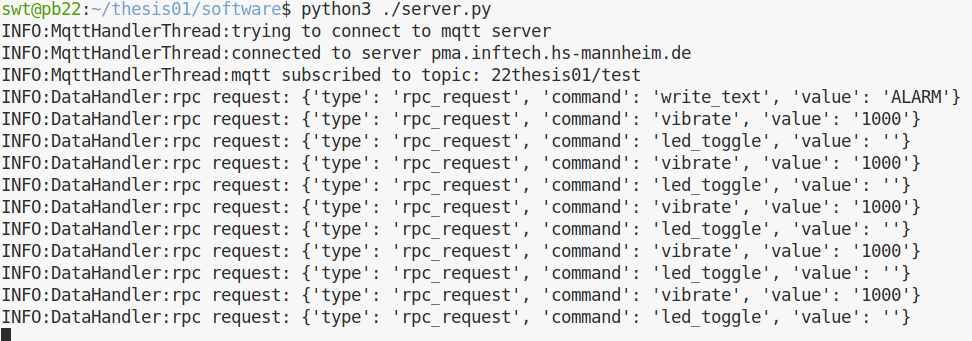
\includegraphics[width=\textwidth]{images/server_requests}
  \caption{Nachrichtenversand der Kontrollanwendung}
  \label{fig:req_controll_app}
\end{figure}
Zu erkennen sind die unterschiedlichen Ausgabekürzel der Anfragen, welche im Feld \texttt{command} abgebildet sind.
Für die Textausgabe entspricht das Kürzel \texttt{write\_text}, für Vibrationen \texttt{vibrate} und für das Umschalten der LED-Farbe \texttt{led\_toggle}.
Pro Ausgabe-Kommando kann zusätzlich ein Parameterwert angegeben werden.
Für \texttt{write\_text} bestimmt er den anzuzeigenden Text und für \texttt{vibrate} die Vibrationsdauer in Millisekunden.
Da es nicht vorgesehen ist die Farbe der Signal-LED manuell festzulegen, wird für \texttt{led\_toggle} kein Parameterwert angegeben.

Wird die App auf dem Smartphone gestartet, befindet Sie sich im Initialmodus in dem Sie bereits Sensorwerte misst und an die Kontrollanwendung sendet.
Das Userinterface ist in Abbildung \ref{fig:initial_app} dargestellt.
\begin{figure}[htbp]
  \centering
  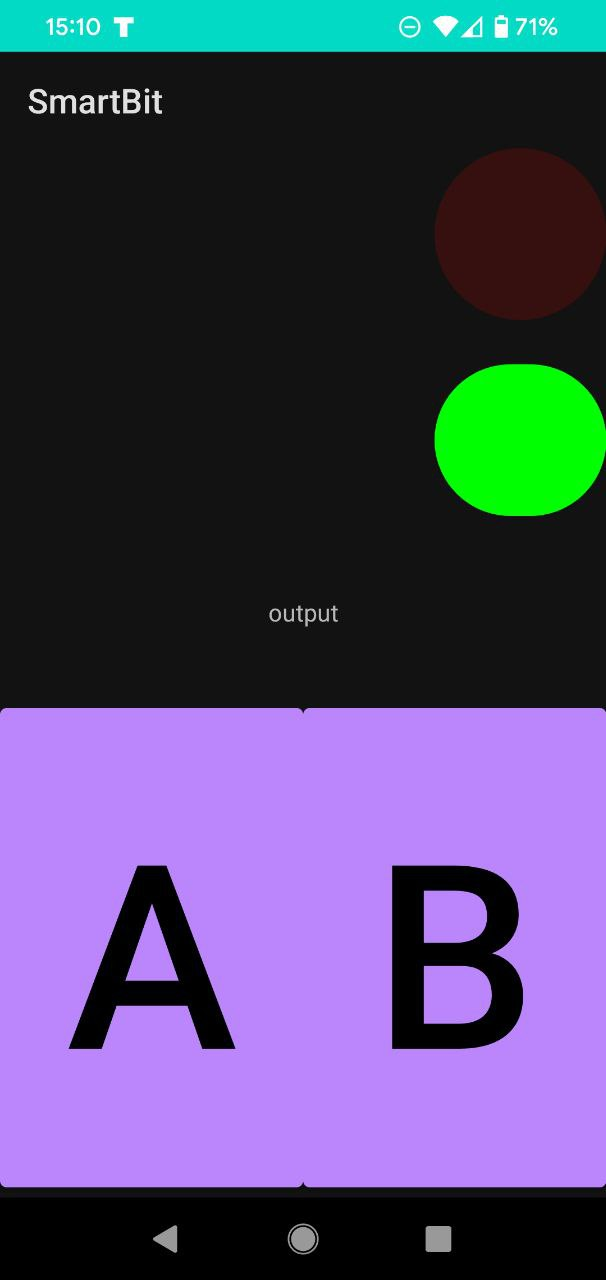
\includegraphics[height=0.4\textheight]{images/app_initial}
  \caption{Initialzustand der mobilen Anwendung}
  \label{fig:initial_app}
\end{figure}
Es besteht aus zwei mit A und B beschrifteten Buttons, einem Textfeld in der Mitte, einer Signal-LED welche zu Beginn grün leuchtet und einer Vorgangs-LED, welche während der Ausführung von Ausgaben aufleuchtet.

Im Alarmfall werden die vom Programm gesendeten Ausgaben entsprechend umgesetzt und das Aussehen des Userinterfaces verändert.
Das Resultat ist in Abbildung \ref{fig:app_alarm} dargestellt.
\begin{figure}[htbp]
  \centering
  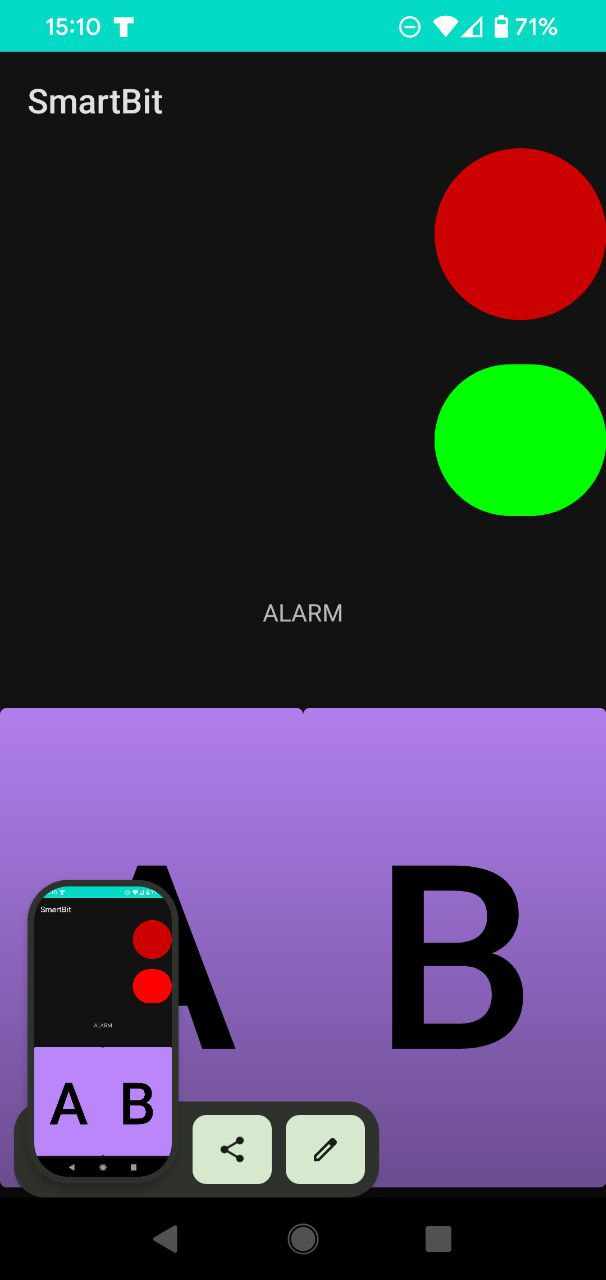
\includegraphics[height=0.4\textheight]{images/app_alarm}
  \caption{Alarmzustand der mobilen Anwendung}
  \label{fig:app_alarm}
\end{figure}
Das Textfeld stellt nun den Text \textit{ALARM} dar und die Farbe der Signal-LED hat sich von grün auf rot geändert.
Die Vorgangs-LED leuchtet rot um zu signalisieren dass gerade eine Ausgabe ausgeführt wird.
Diese ist nicht sichtbar, denn es handelt sich um das haptische Vibrationsfeedback.
% Voraussetzung für die Nutzung der App ist ein Smartphone mit mindestens Android 7 (Nougat [API Level 24])
% Entwickelt wurde Smartbit mit Android Studio Bumblebee (2021.1.1 Patch 2) und Visual Studio Code (v1.68.1).
% Die Bibliotheken und Kontrollanwendung wurden unter Windows 10 (21H1), Windows 11 (21H2) und Debian GNU/Linux 11 (bullseye) unter den Python-Versionen 3.9.0, 3.9.2, 3.10.2, Java 17.0.2 und C18 mit GCC 10.2.1.
% Als JSON-Parser werden unter Java Json for Java (v20220320) und unter C libcjson v1.7.14-1 verwendet.

Nutzerinnen und Nutzer können alle in den Anforderungen aufgestellten Ausgabemöglichkeiten und Sensortypen nutzen.
Implementierte Funktionen kommunizieren zwar mit der Kontrollanwendung in serialisierten Nachrichtenformaten, geben an die aufrufenden Programme jedoch primitive Datentypen zurück.
Die Bibliothek ist portabel nutzbar, da die Stub-Funktionen jeweils für die Programmiersprachen C, Java und Python implementiert wurden.
Eine Einbindung in Eclipse IDE ist möglich, jedoch durch die zusätzlich benötigten JSON-Parser-Bibliotheken für C- und Java-Projekte nicht trivial.
Da Java und Python plattformunabhängige Programmiersprachen sind, erübrigt sich die zweifache Implementierung für Unix- und Windows-Systeme.
Smartbit ermöglicht ein responsives Verhalten der Komponenten.
Im vorangegangen Beispiel \textit{Alarmanlage} betrug die Reaktionszeit unter einer Sekunde.
Smartphoneseitige Latenzen werden architekturbedingt durch die Zwischenspeicherung von Kontrollanwendung verschleiert.
Von Umgebungseigenschaften abhängige Variierungen der Übertragungsgeschwindigkeit ist dadurch für die Programmiererin oder den Programmierer nicht sichtbar.
Mit der Verwendung von MQTT und UDP wurden leichtgewichtige, ihrem Einsatzzweck entsprechende Protokolle für die Kommunikation gewählt.
Trotz der Übertragung mit einem einem QoS-Level 0 werden auch Ausgabeanfragen sicher übertragen und ausgeführt.
Nachrichten, die über die MQTT-Verbindung zwischen Kontrollanwendung und Smartphone-App versandt werden, werden auf dem Übertragungsweg mit TLS verschlüsselt übertragen.
Nachrichten, die über die UDP-Verbindung zwischen Kontrollanwendung und Bibliothek übertragen werden, werden nicht verschlüsselt.
Ein unberechtigtes Mitlesen des Datenverkehrs setzt jedoch voraus, dass Angreifer Nutzerrechte auf dem PC der Nutzerin oder des Nutzers besäßen, da Datagramme lediglich über das Loopback-Interface ausgetauscht werden können.
Das Smartphone ist vor einer \acrfull{rce}-Attacke geschützt, da nur Ausgaben ausgeführt werden können, die von der API spezifiziert wurden.
Smartbit setzt durch die Implementierung von Log-Ausgaben in Kontrollanwendung und Smartphone ebenfalls die Anforderungen an die Transparenz um.

\section{Latenzmessung}
Im Zuge der Konzeption wurden Latenzen eine besondere Bedeutung zugemessen.
Erhöhte Latenzzeiten führen zu einem verzögerten Verhalten und einer schlechteren Benutzbarkeit.
Zum Zwecke der Evaluation der Latenzen werden für drei Nutzungsszenarien Messungen durchgeführt.
Da \texttt{sensor\_requests} lediglich über die Local-Loopback-Schnittstelle zwischen Bibliothek und Kontrollanwendung ausgetauscht werden ist anzunehmen, dass diese Verbindung in der Smartbit-Lösung keine Limitierung darstellt.
Auf die Untersuchung der Latenzzeiten zwischen dem Absenden eines \texttt{sensor\_requests} und dem Erhalt einer \texttt{sensor\_response} wird daher verzichtet.

Unbekannt ist indes die Latenz zwischen Smartphone-App und Kontrollprogramm.
Über diesen Transportweg werden die Nachrichtenformate \texttt{rpc\_request}, \texttt{rpc\_response} und \texttt{update\_request} übermittelt.
Durch die marginale Latenz zwischen Kontrollanwendung und Bibliothek können Sensorwerte zwar häufig abgefragt werden, jedoch wird bis zum Eintreffen eines neuen Sensormesswerts der zuletzt Eingespeicherte zurückgegeben.
Sensordatenabfragen sind daher abhängig von der MQTT-Verbindung zwischen Smartphone und Kontrollanwendung.
Um ein realistisches Nutzungsverhalten zu simulieren, wird für die Messungen der Transportweg zwischen Bibliothek und Smartphone-App betrachtet.
Gemessen wird die Zeitdauer nach Versand eines \texttt{rpc\_requests} bis zum Erhalt einer \texttt{rpc\_response} von der Smartphone-App.
Die Smartphone-App sendet währenddessen fortlaufend \texttt{update\_request}s per MQTT umd reguläre Last auf der Kontrollanwendung zu simulieren.
Messungen finden für drei verschiedene Nutzungsszenarien statt: Der Verwendung im Labor des SWT-Instituts an der Hochschule, der Heimarbeit über eine DSL-Verbindung und der Verwendung in einer virtuellen Umgebung.
Für alle Messungen erfolgen Internetzugriffe seitens des lokalen PCs kabelgebunden und seitens des Smartphones über WLAN.
Die Anzahl der verbunden Geräte des AccessPoints sind für die Übertragungszeit ebenfalls ausschlaggebend.
Die bei CSMA/CA zum Kollisionsschutz verwendeten randomisierten Sendefenster limitieren mit steigender Geräteanzahl die Sendezeit und erhöhen die Latenzen.
Um signifikante Ergebnisse zu diskutieren werden pro Nutzungsszenario 100 Messwerte erhoben und in einem Boxplot dargestellt.

Mit dem SWT-Labor befindet sich der lokale PC im ersten Nutzungsszenario im gleichen Netzbereich wie der MQTT-Broker, was den Transportweg reduziert.
Die Messergebnisse sind in Abbildung \ref{fig:measure_institute} dargestellt.
\begin{figure}[htbp]
  \centering
  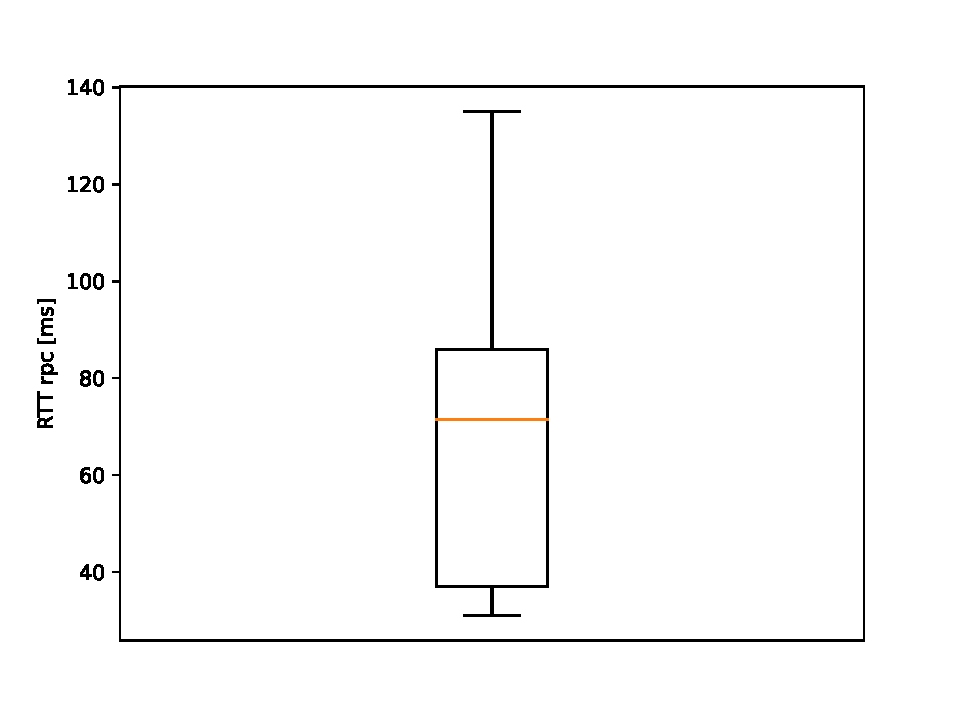
\includegraphics[width=0.7\textwidth]{images/timing_institute.pdf}
  \caption{Messergnisse der Latenzmessungen im Heimnetz}
  \label{fig:measure_institute}
\end{figure}
Die Latenzen sind mit Maximalwerten von 138 ms sehr gering  
SensorEventListener erheben Daten mit einer eine Verzögerung von maximal 200 ms.
Hier könnte auch die eigentliche Sensormessung auf dem Smartphone die Übertragungsgeschwindigkeit begrenzen.
Im Labor-Szenario kann die Smartbit-Lösung eingesetzt werden.

Die Messung des zweiten Szenarios erfolgt aus einem Heimnetz mit acht Hops zwischen Broker und lokalem PC. 
Auf dem Access Point sind zur Zeit der Messung acht Geräte registriert.
Die Messergebnisse sind relevant für die Heimarbeit oder für die Verwendung beim Erledigen von Hausaufgaben.
Die Ergebnisse sind in Abbildung \ref{fig:measure_home} dargestellt.
\begin{figure}[htbp]
  \centering
  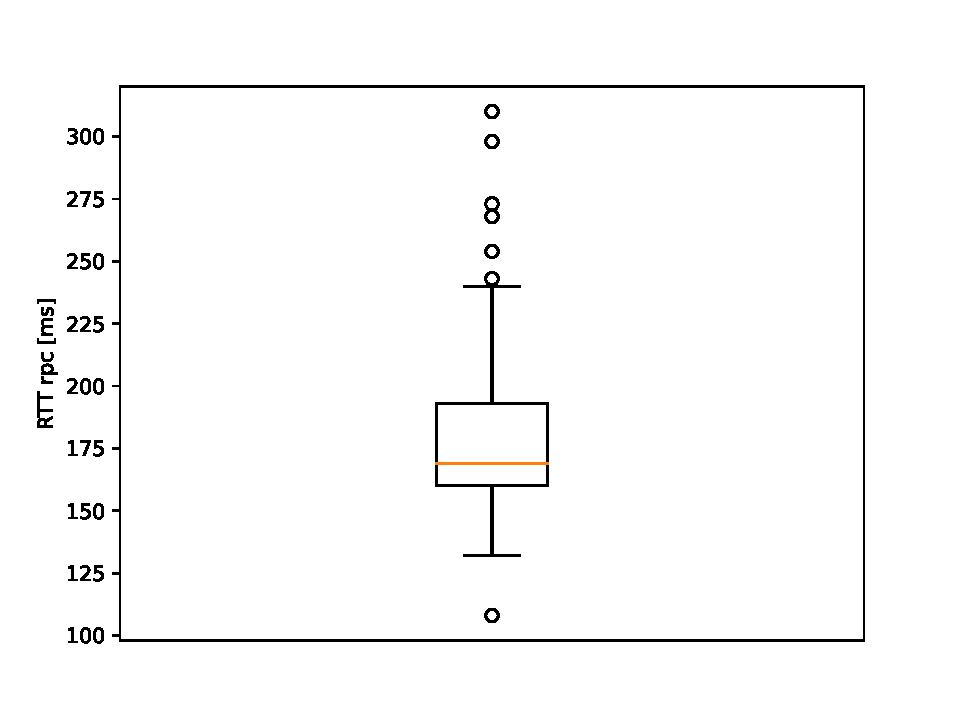
\includegraphics[width=0.7\textwidth]{images/timing_at_home}
  \caption{Messergebnisse der Latenzmessungen im Heimnetz}
  \label{fig:measure_home}
\end{figure}
Die Messwerte fallen mit einem Median von etwa 175 ms deutlich höher als im Labor aus, befinden sich allerdings immer noch im tolerablen Bereich und stellen keine gravierende Beeinträchtigung in der Benutzung der Smartbit-Lösung dar.

Im dritten Szenario wird die Messung von einer in VirtualBox gestarteten, virtuellen Maschine auf dem lokalen PC aus gestartet.
Sowohl Bibliothek und Kontrollanwendung werden in der virtuellen Maschine betrieben.
Relevant ist das Szenario ebenfalls für die Heimarbeit.
Es bildet die Verwendung der virtuellen Maschine zum Programmieren ab.
In den Lehrveranstaltungen des Instituts wird dies häufig angewandt um Studierenden auf simplem Wege eine vollständige Programmierumgebung zur Verfügung zu stellen. 
Untersucht wird, ob die Latenzzeiten sich durch die NAT-Funktionalität von VirtualBox signifikant vergrößern.
Die Messergebnisse sind in Abbildung \ref{fig:measure_vm} dargestellt.
\begin{figure}[htbp]
  \centering
  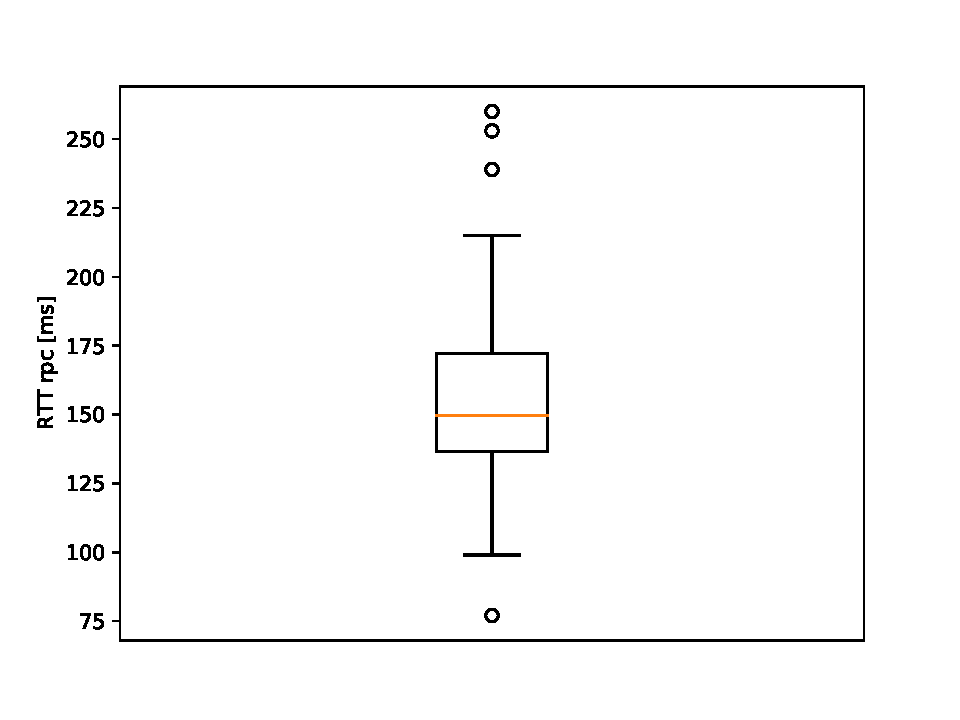
\includegraphics[width=0.6\textwidth]{images/timing_vm}
  \caption{Messergebnisse der Latenzmessungen im Heimnetz}
  \label{fig:measure_vm}
\end{figure}
Die Latenzzeiten sind im Vergleich zur Messung auf dem Host-PC nicht wesentlich angestiegen.
Dadurch ist ebenfalls von keiner maßgeblichen Beeinträchtigung der Nutzung auszugehen.
Sie kann auch in virtuellen Entwicklungsumgebungen verwendet werden.

\chapter{Fazit}\label{chap:fazit}
Die Smartbit-Lösung erfüllt die Anforderungen zufriedenstellend.
Die im Vorfeld durchgeführte Konzeption ermöglichte eine problemlose Implementierung.
Während der Entwicklung wurden jedoch einige Designentscheidungen getroffen, welche die Smartbit-Lösung beschränken.
Sensordaten werden von der Kontrollanwendung nicht für einzelne Geräte eingespeichert.
Es ist nicht möglich, Programmcode simultan auf mehreren Smartphones gleichzeitig auszuführen.
Gruppen-Sessions können nicht erstellt werden.
Für Programme die die Java und Python-Schnittstelle erscheint dies kontraintuitiv.
Die Bedeutung eines Phone-Objektes lässt auf eine zwischen Einzelgeräten unterscheidende Verwendung schließen.
Ein weiterer Nachteil der Benutzerfreundlichkeit besteht in der zwingenden Verwendung von Hilfs-Bibliotheken für den Nachrichtenaustausch über JSON.
Sowohl für Java, als auch für C sind zusätzliche JSON-Parser für die Kommunikation zwischen Bibliothek und Kontrollanwendung nötig.
Für eine erfolgreiche Kompilierung in C muss der Dateipfad für diesen dem Linker bekannt gemacht werden.
Für die interne Struktur ist die Datenverwaltung innerhalb des Programms ausreichend.
Durch den asynchronen Ansatz des Multithreading können beide Kommunikationspartner gleichzeitig über das Kontrollprogramm kommunizieren und zwischengespeicherte Daten auslesen oder bearbeiten.
Die Möglichkeit, mehrere Werte zum internen Datenspeicher hinzuzufügen, wird jedoch nicht unterstützt.
Häufige Sensor-Anfragen werden mit dem gleichen, einzeln zwischengespeicherten Sensorwert beantwortet, welcher zusätzlich kein Ablaufdatum besitzt.
Abbrüche der Übertragung resultieren in der kontinuierlichen Übermittlung des zuletzt eingespeicherten Sensorwerts.

Zur Ablösung von Hilfsbibliotheken eignet sich die Verwendung eines Binärprotokolls.
In Enumerationen konvertierte Nachrichtenformate und Parameter könnten statt der implementierten Darstellung mit JSON eingesetzt werden.
Dadurch entfiele nicht nur der Nachteil der kontraintuitiv Einbindung.
Die Nachrichtengröße würde ebenfalls verringert werden.
Energieeffizienz der Android-App wurde zum Vorteil der Latenzreduzierung während der Implementierung nicht wesentlich berücksichtigt.
Zum Start der Anwendung werden die Sensormessprozesse unmittelbar gestartet und Sensorwerte an die Kontrollanwendung gesendet, was einen erhöhten Energieverbrauch bedeutet.
Sollten sich die Startzeiten der Sensormessprozesse nicht wesentlich auf die Latenzen auswirken, wäre eine auf Anfragen basierende Sensormessdatenübertragung erwägenswert, um den Energieverbrauch zu reduzieren.

% Listen wenn überhaupt ans Ende und nicht an den Anfang.
% Meist ist das aber unnötig.
% List of abbrev
\listoffigures % Liste der Abbildungen 
\listoftables % Liste der Tabellen
\printglossary[type=\acronymtype, title={Abkürzungsverzeichnis}, nonumberlist=true]

\newpage

%check: hat das hier geklappt?


\bibliographystyle{plain} % Literaturverzeichnis
\begin{btSect}{thesis} % mit bibtopic Quellen trennen
\addcontentsline{toc}{chapter}{Literaturverzeichnis und Online-Quellen}
\section*{Literaturverzeichnis}
\btPrintCited
\end{btSect}
\begin{btSect}{online}
\section*{Online-Quellen}
\btPrintCited
%\bibliography{online}
\end{btSect}
% dann mit "bibtex thesis1" und "bibtex thesis2" arbeiten

\appendix
\chapter{Nachrichtenformate}
\lstset{language=python, captionpos=b, frame=single, numberstyle=\tiny, style=customcs}
\lstinputlisting[caption=Update-Request]{listings/messages/update_request.json}
\lstinputlisting[caption=Sensor-Request]{listings/messages/sensor_request.json}
\lstinputlisting[caption=Sensor-Response]{listings/messages/sensor_response.json}
\lstinputlisting[caption=RPC-Request]{listings/messages/sensor_request.json}
\lstinputlisting[caption=RPC-Response]{listings/messages/sensor_response.json}


\end{document}
;;; Local Variables:
;;; ispell-local-dictionary: "de_DE-neu"
;;; End:


